\documentclass[twoside]{book}

% Packages required by doxygen
\usepackage{fixltx2e}
\usepackage{calc}
\usepackage{doxygen}
\usepackage{graphicx}
\usepackage[utf8]{inputenc}
\usepackage{makeidx}
\usepackage{multicol}
\usepackage{multirow}
\PassOptionsToPackage{warn}{textcomp}
\usepackage{textcomp}
\usepackage[nointegrals]{wasysym}
\usepackage[table]{xcolor}

% Font selection
\usepackage[T1]{fontenc}
\usepackage{mathptmx}
\usepackage[scaled=.90]{helvet}
\usepackage{courier}
\usepackage{amssymb}
\usepackage{sectsty}
\renewcommand{\familydefault}{\sfdefault}
\allsectionsfont{%
  \fontseries{bc}\selectfont%
  \color{darkgray}%
}
\renewcommand{\DoxyLabelFont}{%
  \fontseries{bc}\selectfont%
  \color{darkgray}%
}
\newcommand{\+}{\discretionary{\mbox{\scriptsize$\hookleftarrow$}}{}{}}

% Page & text layout
\usepackage{geometry}
\geometry{%
  a4paper,%
  top=2.5cm,%
  bottom=2.5cm,%
  left=2.5cm,%
  right=2.5cm%
}
\tolerance=750
\hfuzz=15pt
\hbadness=750
\setlength{\emergencystretch}{15pt}
\setlength{\parindent}{0cm}
\setlength{\parskip}{0.2cm}
\makeatletter
\renewcommand{\paragraph}{%
  \@startsection{paragraph}{4}{0ex}{-1.0ex}{1.0ex}{%
    \normalfont\normalsize\bfseries\SS@parafont%
  }%
}
\renewcommand{\subparagraph}{%
  \@startsection{subparagraph}{5}{0ex}{-1.0ex}{1.0ex}{%
    \normalfont\normalsize\bfseries\SS@subparafont%
  }%
}
\makeatother

% Headers & footers
\usepackage{fancyhdr}
\pagestyle{fancyplain}
\fancyhead[LE]{\fancyplain{}{\bfseries\thepage}}
\fancyhead[CE]{\fancyplain{}{}}
\fancyhead[RE]{\fancyplain{}{\bfseries\leftmark}}
\fancyhead[LO]{\fancyplain{}{\bfseries\rightmark}}
\fancyhead[CO]{\fancyplain{}{}}
\fancyhead[RO]{\fancyplain{}{\bfseries\thepage}}
\fancyfoot[LE]{\fancyplain{}{}}
\fancyfoot[CE]{\fancyplain{}{}}
\fancyfoot[RE]{\fancyplain{}{\bfseries\scriptsize Generated on Fri Mar 31 2017 16\+:31\+:26 for Root Data Reader by Doxygen }}
\fancyfoot[LO]{\fancyplain{}{\bfseries\scriptsize Generated on Fri Mar 31 2017 16\+:31\+:26 for Root Data Reader by Doxygen }}
\fancyfoot[CO]{\fancyplain{}{}}
\fancyfoot[RO]{\fancyplain{}{}}
\renewcommand{\footrulewidth}{0.4pt}
\renewcommand{\chaptermark}[1]{%
  \markboth{#1}{}%
}
\renewcommand{\sectionmark}[1]{%
  \markright{\thesection\ #1}%
}

% Indices & bibliography
\usepackage{natbib}
\usepackage[titles]{tocloft}
\setcounter{tocdepth}{3}
\setcounter{secnumdepth}{5}
\makeindex

% Hyperlinks (required, but should be loaded last)
\usepackage{ifpdf}
\ifpdf
  \usepackage[pdftex,pagebackref=true]{hyperref}
\else
  \usepackage[ps2pdf,pagebackref=true]{hyperref}
\fi
\hypersetup{%
  colorlinks=true,%
  linkcolor=blue,%
  citecolor=blue,%
  unicode%
}

% Custom commands
\newcommand{\clearemptydoublepage}{%
  \newpage{\pagestyle{empty}\cleardoublepage}%
}


%===== C O N T E N T S =====

\begin{document}

% Titlepage & ToC
\hypersetup{pageanchor=false,
             bookmarks=true,
             bookmarksnumbered=true,
             pdfencoding=unicode
            }
\pagenumbering{roman}
\begin{titlepage}
\vspace*{7cm}
\begin{center}%
{\Large Root Data Reader }\\
\vspace*{1cm}
{\large Generated by Doxygen 1.8.8}\\
\vspace*{0.5cm}
{\small Fri Mar 31 2017 16:31:26}\\
\end{center}
\end{titlepage}
\clearemptydoublepage
\tableofcontents
\clearemptydoublepage
\pagenumbering{arabic}
\hypersetup{pageanchor=true}

%--- Begin generated contents ---
\chapter{Main Page}
\label{index}\hypertarget{index}{}Simple reader and (not only \href{http://json.org/}{\tt J\+S\+O\+N}) serializer build on \href{https://github.com/miloyip/rapidjson}{\tt rapidjson} for data in \href{https://root.cern.ch/}{\tt R\+O\+O\+T} scientific framework format.

\paragraph*{\href{https://jiri-vyc.github.io/rootdatareader/docs/}{\tt Source documentation here}}

\subsubsection*{What is this project good for?}

This project is aimed for developers who have to or want to work with any arbitrary data stored in \href{http://home.cern/}{\tt C\+E\+R\+N}'s \href{https://root.cern.ch/}{\tt R\+O\+O\+T} format without writing complicated proprietary readers, converters and such. This project lets you simply define format of the data, and read them. Without the hassle.

Motivation was increasing popularity of web visualization tools that work with and display scientific data originally stored in the R\+O\+O\+T format. Goal was to provide simple and general way how to read the R\+O\+O\+T data in {\itshape any} format and get them to Java\+Script in the most convenient format (read J\+S\+O\+N).

\subsubsection*{Simple usage example}


\begin{DoxyCode}
\hyperlink{classRootDataDefinition}{RootDataDefinition} * definition;        \textcolor{comment}{// General definition of data }
\hyperlink{classRootDataReader}{RootDataReader} * dataReader;            \textcolor{comment}{// The reader}
dataReader = \textcolor{keyword}{new} \hyperlink{classRootDataReader}{RootDataReader}();      \textcolor{comment}{// Initialize}
definition = \textcolor{keyword}{new} \hyperlink{classOnlyToADataDefinition}{OnlyToADataDefinition}(\textcolor{stringliteral}{"data/testFile1.root"}, \textcolor{stringliteral}{"Datatree"});  \textcolor{comment}{//
       Initializing concrete data definition}

dataReader->\hyperlink{classRootDataReader_ad670745df69f90ea6578d7c29cab716f}{SetDataDefinition}(definition);  \textcolor{comment}{// Tell the reader to use this data definition}

cout << dataReader->\hyperlink{classRootDataReader_a76a02dd2cc6f4cde896ce9180048671b}{GetInterval}(0, 5)->\hyperlink{classDataEntryInterval_ad27bffbb603c300714090c809ee58570}{JSONify}() << endl;
\end{DoxyCode}
 This will nicely, simply print (interval of entries on indexes 0 to 5)\+: 
\begin{DoxyCode}
\{
  \textcolor{stringliteral}{"Size"}:5,
  \textcolor{stringliteral}{"Entries"}:[
    \{\textcolor{stringliteral}{"ToA"}:481258120.3125\},\{\textcolor{stringliteral}{"ToA"}:481258120.3125\},\{\textcolor{stringliteral}{"ToA"}:481258120.3125\},\{\textcolor{stringliteral}{"ToA"}:481258120.3125\},\{\textcolor{stringliteral}{"ToA"}:
      481258120.3125\}
  ]
\}
\end{DoxyCode}
 \subsubsection*{So how does it work and how do I use it for my data?}

There are three main components of the project\+:


\begin{DoxyItemize}
\item \hyperlink{classRootDataReader}{Root\+Data\+Reader}

Leave this class as is, use its A\+P\+I to your heart's content. One of its method is \hyperlink{classRootDataReader_ad670745df69f90ea6578d7c29cab716f}{Root\+Data\+Reader\+::\+Set\+Data\+Definition()}, where you assign the definition, where the data you want to read are and what structure do they have. Its only parameter has to be of type \hyperlink{classRootDataDefinition}{Root\+Data\+Definition}.
\item \hyperlink{classRootDataDefinition}{Root\+Data\+Definition}

This is where the definition of the data happens. It describes which data, where, and how they are stored in the root file. It describes the types and names of the branches you will be working with. It is an abstract class and only dictates you which methods you have to have in your child class. Extend this class, define the types and names of values you will have in your data (see example \hyperlink{classOnlyToADataDefinition}{Only\+To\+A\+Data\+Definition}). Each of the values represent a single value stored in the tree branch and will be automatically filled. Then, implement the Get\+Entry() method. In this method, manipulate the values from the branches that you specified as you want and save the result into object of type \hyperlink{classSingleDataEntry}{Single\+Data\+Entry} and return it.
\item \hyperlink{classSingleDataEntry}{Single\+Data\+Entry}

This is the class which represents one single data object you want to be working with. It doesn't have to correspond 1\+:1 with the data stored in root files and defined in \hyperlink{classRootDataDefinition}{Root\+Data\+Definition}. You have stored 2 parts of the desired object's single attribute in 2 separate branches? No problem, combine them in defined way in the \hyperlink{classRootDataDefinition}{Root\+Data\+Definition} and store them in single value in \hyperlink{classSingleDataEntry}{Single\+Data\+Entry}. This is the resulting object (representing real one) that you want to be manipulating, visualizing, evaluating. No matter how the data are physically stored in the files. It can be complex particle cluster, a frame, or a simple object with only one value (as in example \hyperlink{classSinglePixelToA}{Single\+Pixel\+To\+A}). To get such object, extend this class (\hyperlink{classSingleDataEntry}{Single\+Data\+Entry}), define your concrete entry's attributes, implement your own Getters and Setters if needed and implement the virtual methods Print() and J\+S\+O\+Nify(), specifying, how you want to print/serialize your values (you can see example in \hyperlink{classSinglePixelToA_a8b9d4ef4082473c747157b9b2c1376b0}{Single\+Pixel\+To\+A\+::\+Print()} and \hyperlink{classSingleDataEntry_a9e48725016d6fbd6bd674d5b299dbb12}{Single\+Pixel\+To\+A\+::\+J\+S\+O\+Nify()}).

You can have data stored in two different ways (different trees, different branches), but you want to get the same resulting data from them? No problem either, you can have several different Root\+Data\+Definitions, which define and manipulate the data in different way, but stores them into single (same) \hyperlink{classSingleDataEntry}{Single\+Data\+Entry}. Later you can work with these objects exactly the same way, they are the same object, no matter where they came from.

The other way around? Also no problem, define two Root\+Data\+Definitions to read the exact same data, but save them into different (\hyperlink{classSingleDataEntry}{Single\+Data\+Entry}) objects.
\end{DoxyItemize}

\subsubsection*{So what can I do with it then?}

For example this\+:


\begin{DoxyCode}
dataReader = \textcolor{keyword}{new} \hyperlink{classRootDataReader}{RootDataReader}();      \textcolor{comment}{// Initialize}
definition = \textcolor{keyword}{new} TPX3HitDataDefinition(\textcolor{stringliteral}{"data/testFile1.root"}, \textcolor{stringliteral}{"Datatree"});  \textcolor{comment}{// Initializing concrete data
       definition}

dataReader->\hyperlink{classRootDataReader_ad670745df69f90ea6578d7c29cab716f}{SetDataDefinition}(definition);  \textcolor{comment}{// Tell the reader to use this data definition}

cout << dataReader->GetEntry(0)->JSONify() << endl;
\end{DoxyCode}


Prints\+:


\begin{DoxyCode}
\{\textcolor{stringliteral}{"index"}: 0, \textcolor{stringliteral}{"PixX"}: 250, \textcolor{stringliteral}{"PixY"}: 154, \textcolor{stringliteral}{"ToT"}: 332, \textcolor{stringliteral}{"ToA"}:481258120.3125, \textcolor{stringliteral}{"triggerNo"}: 0\}
\end{DoxyCode}


And adding this\+:


\begin{DoxyCode}
definition2 = \textcolor{keyword}{new} TPX3ClusterDataDefinition(\textcolor{stringliteral}{"data/testFile1.root"}, \textcolor{stringliteral}{"Clustertree"});
dataReader->\hyperlink{classRootDataReader_ad670745df69f90ea6578d7c29cab716f}{SetDataDefinition}(definition2);

cout << dataReader->GetEntry(0)->JSONify() << endl;
\end{DoxyCode}


Prints\+:


\begin{DoxyCode}
\{
    \textcolor{stringliteral}{"clstrSize"}: 3, 
    \textcolor{stringliteral}{"PixX"}: [250, 102, 51], 
    \textcolor{stringliteral}{"PixY"}: [154, 252, 189], 
    \textcolor{stringliteral}{"ToT"}: [332, 12, 105], 
    \textcolor{stringliteral}{"ToA"}: [481258120.3125, 481258200.625, 481258220.0], 
    \textcolor{stringliteral}{"clstrType"}: \textcolor{stringliteral}{"Small Blob"}, 
    \textcolor{stringliteral}{"clstrVolCentroidX"}: 110, 
    \textcolor{stringliteral}{"clstrVolCentroidY"}: 188
\}
\end{DoxyCode}


\subsubsection*{Also it can do sorting \& binary search!}

You just have to specify primary sorted branch of the used tree in the \hyperlink{classRootDataDefinition}{Root\+Data\+Definition} class and the \hyperlink{classRootDataReader}{Root\+Data\+Reader} does everything for you. You provide the value you want to find, and the reader will use its native, fast binary search algorithm to find the index on which this value in the tree/root file is. With any type of the data definition, with any (comparable by $<$) type of the branch value. Use like this\+:

Specify that the primary branch, which is sorted and by which the searching will happen, is the \char`\"{}\+To\+A\char`\"{} branch\+: 
\begin{DoxyCode}
\textcolor{keywordtype}{void} * \hyperlink{classOnlyToADataDefinition_af2025f39b59dc8bd50a281f5034ed47a}{OnlyToADataDefinition::GetPrimarySortedBranch}()\{
    \textcolor{keywordflow}{return} (\textcolor{keywordtype}{void}*)this->ToA;
\}
\end{DoxyCode}


and then just search for specific value (and specify its type)


\begin{DoxyCode}
cout << \textcolor{stringliteral}{"Index: "} << dataReader->\hyperlink{classRootDataReader_a04d8033b9761cc8c673af9bb96adfc03}{GetStartingIndex}<Double\_t>(481258120) << endl;
\end{DoxyCode}


and the result is the index on which the values of the \char`\"{}\+To\+A\char`\"{} branch start to be bigger than 481258120, found by binary search.

\subsubsection*{How to set it up and use it?}

You need only few prerequisites\+:


\begin{DoxyItemize}
\item R\+O\+O\+T Installed
\item g++ 4.\+9+
\item make
\end{DoxyItemize}

There is a Makefile included in the project, so all you have to do to compile the example is to run {\ttfamily make} in the project's folder.

When you add your classes and implementations, add them to the Makefile\+:


\begin{DoxyCode}
1 rootdatareader: main.o reader.o definition.o pixeltoa.o definitiontoa.o interval.o mynewclass.o
2 mynewclass.o:
3     $(CC) $(CFLAGS) src/MyNewClass.cpp -o build/MyNewClass.o
\end{DoxyCode}


\subsubsection*{Contribution guidelines}


\begin{DoxyItemize}
\item T\+O\+D\+O
\end{DoxyItemize}

\subsubsection*{Who do I talk to?}

\href{mailto:jiri.vyc@gmail.com}{\tt jiri.\+vyc@gmail.\+com} 
\chapter{Hierarchical Index}
\section{Class Hierarchy}
This inheritance list is sorted roughly, but not completely, alphabetically\+:\begin{DoxyCompactList}
\item \contentsline{section}{Data\+Entry\+Interval}{\pageref{classDataEntryInterval}}{}
\item \contentsline{section}{Root\+Data\+Definition}{\pageref{classRootDataDefinition}}{}
\begin{DoxyCompactList}
\item \contentsline{section}{Only\+To\+A\+Data\+Definition}{\pageref{classOnlyToADataDefinition}}{}
\end{DoxyCompactList}
\item \contentsline{section}{Root\+Data\+Reader}{\pageref{classRootDataReader}}{}
\item \contentsline{section}{Single\+Data\+Entry}{\pageref{classSingleDataEntry}}{}
\begin{DoxyCompactList}
\item \contentsline{section}{Single\+Pixel\+To\+A}{\pageref{classSinglePixelToA}}{}
\end{DoxyCompactList}
\end{DoxyCompactList}

\chapter{Class Index}
\section{Class List}
Here are the classes, structs, unions and interfaces with brief descriptions\+:\begin{DoxyCompactList}
\item\contentsline{section}{\hyperlink{classDataEntryInterval}{Data\+Entry\+Interval} \\*The class representing an interval of root data entries }{\pageref{classDataEntryInterval}}{}
\item\contentsline{section}{\hyperlink{classOnlyToADataDefinition}{Only\+To\+A\+Data\+Definition} \\*Class defining the structure of data within root file containing only one value (of type double) -\/ To\+A }{\pageref{classOnlyToADataDefinition}}{}
\item\contentsline{section}{\hyperlink{classRootDataDefinition}{Root\+Data\+Definition} \\*Abstract interface for defining a structure of the data in the R\+O\+O\+T files, process how to read these data and save them to desired data objects }{\pageref{classRootDataDefinition}}{}
\item\contentsline{section}{\hyperlink{classRootDataReader}{Root\+Data\+Reader} \\*Class responsible for reading data of various structure in the R\+O\+O\+T format (T\+Tree within T\+File) }{\pageref{classRootDataReader}}{}
\item\contentsline{section}{\hyperlink{classSingleDataEntry}{Single\+Data\+Entry} \\*Abstract class representing a data object to be retrieved from the R\+O\+O\+T file }{\pageref{classSingleDataEntry}}{}
\item\contentsline{section}{\hyperlink{classSinglePixelToA}{Single\+Pixel\+To\+A} \\*Class defining the data object containing only single value (of type double) -\/ To\+A }{\pageref{classSinglePixelToA}}{}
\end{DoxyCompactList}

\chapter{File Index}
\section{File List}
Here is a list of all files with brief descriptions\+:\begin{DoxyCompactList}
\item\contentsline{section}{src/\hyperlink{DataEntryInterval_8cpp}{Data\+Entry\+Interval.\+cpp} }{\pageref{DataEntryInterval_8cpp}}{}
\item\contentsline{section}{src/\hyperlink{DataEntryInterval_8h}{Data\+Entry\+Interval.\+h} }{\pageref{DataEntryInterval_8h}}{}
\item\contentsline{section}{src/\hyperlink{main_8cpp}{main.\+cpp} }{\pageref{main_8cpp}}{}
\item\contentsline{section}{src/\hyperlink{OnlyToADataDefinition_8cpp}{Only\+To\+A\+Data\+Definition.\+cpp} }{\pageref{OnlyToADataDefinition_8cpp}}{}
\item\contentsline{section}{src/\hyperlink{OnlyToADataDefinition_8h}{Only\+To\+A\+Data\+Definition.\+h} }{\pageref{OnlyToADataDefinition_8h}}{}
\item\contentsline{section}{src/\hyperlink{RootDataDefinition_8cpp}{Root\+Data\+Definition.\+cpp} }{\pageref{RootDataDefinition_8cpp}}{}
\item\contentsline{section}{src/\hyperlink{RootDataDefinition_8h}{Root\+Data\+Definition.\+h} }{\pageref{RootDataDefinition_8h}}{}
\item\contentsline{section}{src/\hyperlink{RootDataReader_8cpp}{Root\+Data\+Reader.\+cpp} }{\pageref{RootDataReader_8cpp}}{}
\item\contentsline{section}{src/\hyperlink{RootDataReader_8h}{Root\+Data\+Reader.\+h} }{\pageref{RootDataReader_8h}}{}
\item\contentsline{section}{src/\hyperlink{SingleDataEntry_8h}{Single\+Data\+Entry.\+h} }{\pageref{SingleDataEntry_8h}}{}
\item\contentsline{section}{src/\hyperlink{SinglePixelToA_8cpp}{Single\+Pixel\+To\+A.\+cpp} }{\pageref{SinglePixelToA_8cpp}}{}
\item\contentsline{section}{src/\hyperlink{SinglePixelToA_8h}{Single\+Pixel\+To\+A.\+h} }{\pageref{SinglePixelToA_8h}}{}
\end{DoxyCompactList}

\chapter{Class Documentation}
\hypertarget{classDataEntryInterval}{\section{Data\+Entry\+Interval Class Reference}
\label{classDataEntryInterval}\index{Data\+Entry\+Interval@{Data\+Entry\+Interval}}
}


The class representing an interval of root data entries.  




{\ttfamily \#include $<$Data\+Entry\+Interval.\+h$>$}



Collaboration diagram for Data\+Entry\+Interval\+:
\nopagebreak
\begin{figure}[H]
\begin{center}
\leavevmode
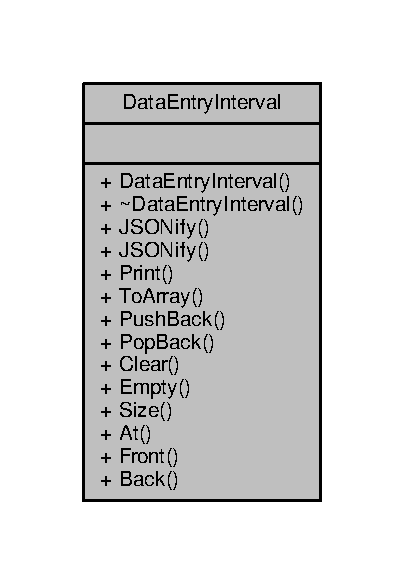
\includegraphics[width=194pt]{classDataEntryInterval__coll__graph}
\end{center}
\end{figure}
\subsection*{Public Member Functions}
\begin{DoxyCompactItemize}
\item 
\hyperlink{classDataEntryInterval_ac3313356193f881b1bbf2e072523db82}{Data\+Entry\+Interval} ()
\begin{DoxyCompactList}\small\item\em Creates an empty interval of size 0. \end{DoxyCompactList}\item 
\hyperlink{classDataEntryInterval_a4b446c378e1ad0a5f63b5d131090f384}{$\sim$\+Data\+Entry\+Interval} ()
\begin{DoxyCompactList}\small\item\em Destroys the object and disposes of all the data contained within. \end{DoxyCompactList}\item 
std\+::string \hyperlink{classDataEntryInterval_ad27bffbb603c300714090c809ee58570}{J\+S\+O\+Nify} ()
\begin{DoxyCompactList}\small\item\em Returns all the data from the interval in form of a string-\/encoded J\+S\+O\+N object. \end{DoxyCompactList}\item 
void \hyperlink{classDataEntryInterval_aba5c55640085036f23b3a1afb2db3a15}{J\+S\+O\+Nify} (rapidjson\+::\+Writer$<$ rapidjson\+::\+String\+Buffer $>$ \&writer)
\begin{DoxyCompactList}\small\item\em Sends all the data from interval to the specified J\+S\+O\+N Writer object. \end{DoxyCompactList}\item 
void \hyperlink{classDataEntryInterval_a869d48a5a8f4562f3f2a5226451f65a2}{Print} ()
\begin{DoxyCompactList}\small\item\em Browse the data contained within this interval in the same fashion, as R\+O\+O\+T's Browse() function. Shows 25 lines of complete data, then queries user if they want to show more. \end{DoxyCompactList}\item 
\hyperlink{classSingleDataEntry}{Single\+Data\+Entry} $\ast$$\ast$ \hyperlink{classDataEntryInterval_a74c1d8cbede885e46afcce933f3adc70}{To\+Array} ()
\begin{DoxyCompactList}\small\item\em Converts to a classic array. \end{DoxyCompactList}\item 
void \hyperlink{classDataEntryInterval_ab8fedb5a71c6203463eaf71bb0f8fa80}{Push\+Back} (\hyperlink{classSingleDataEntry}{Single\+Data\+Entry} $\ast$elem)
\begin{DoxyCompactList}\small\item\em std\+::vector's functionality of the method of the same name \end{DoxyCompactList}\item 
void \hyperlink{classDataEntryInterval_aaa530c4fce5fbddd8ba2b9ed46d30b23}{Pop\+Back} ()
\begin{DoxyCompactList}\small\item\em std\+::vector's functionality of the method of the same name \end{DoxyCompactList}\item 
void \hyperlink{classDataEntryInterval_a24cf69487028f0fd83b693a7d146c4a5}{Clear} ()
\begin{DoxyCompactList}\small\item\em std\+::vector's functionality of the method of the same name \end{DoxyCompactList}\item 
bool \hyperlink{classDataEntryInterval_ab6096bc44c3413423907ee907b789536}{Empty} ()
\begin{DoxyCompactList}\small\item\em std\+::vector's functionality of the method of the same name \end{DoxyCompactList}\item 
unsigned int \hyperlink{classDataEntryInterval_af6be4d0b022e44ec058e16a5bfbefb1e}{Size} ()
\begin{DoxyCompactList}\small\item\em std\+::vector's functionality of the method of the same name \end{DoxyCompactList}\item 
\hyperlink{classSingleDataEntry}{Single\+Data\+Entry} $\ast$ \hyperlink{classDataEntryInterval_a57abfacd1fe9fc36c55c5c4b8a17e62b}{At} (unsigned int position)
\begin{DoxyCompactList}\small\item\em std\+::vector's functionality of the method of the same name \end{DoxyCompactList}\item 
\hyperlink{classSingleDataEntry}{Single\+Data\+Entry} $\ast$ \hyperlink{classDataEntryInterval_ad894e331cac1b4c9ac63957c79022b3d}{Front} ()
\begin{DoxyCompactList}\small\item\em std\+::vector's functionality of the method of the same name \end{DoxyCompactList}\item 
\hyperlink{classSingleDataEntry}{Single\+Data\+Entry} $\ast$ \hyperlink{classDataEntryInterval_a3756bd415ccbdd7db56a2a753c78efaf}{Back} ()
\begin{DoxyCompactList}\small\item\em std\+::vector's functionality of the method of the same name \end{DoxyCompactList}\end{DoxyCompactItemize}


\subsection{Detailed Description}
The class representing an interval of root data entries. 

It is a decorator over the std\+::vector class, as it provides the same functionality of the vector collection and only adds some basic function and J\+S\+O\+N serialization 

Definition at line 14 of file Data\+Entry\+Interval.\+h.



\subsection{Constructor \& Destructor Documentation}
\hypertarget{classDataEntryInterval_ac3313356193f881b1bbf2e072523db82}{\index{Data\+Entry\+Interval@{Data\+Entry\+Interval}!Data\+Entry\+Interval@{Data\+Entry\+Interval}}
\index{Data\+Entry\+Interval@{Data\+Entry\+Interval}!Data\+Entry\+Interval@{Data\+Entry\+Interval}}
\subsubsection[{Data\+Entry\+Interval}]{\setlength{\rightskip}{0pt plus 5cm}Data\+Entry\+Interval\+::\+Data\+Entry\+Interval (
\begin{DoxyParamCaption}
{}
\end{DoxyParamCaption}
)\hspace{0.3cm}{\ttfamily [inline]}}}\label{classDataEntryInterval_ac3313356193f881b1bbf2e072523db82}


Creates an empty interval of size 0. 



Definition at line 20 of file Data\+Entry\+Interval.\+h.

\hypertarget{classDataEntryInterval_a4b446c378e1ad0a5f63b5d131090f384}{\index{Data\+Entry\+Interval@{Data\+Entry\+Interval}!````~Data\+Entry\+Interval@{$\sim$\+Data\+Entry\+Interval}}
\index{````~Data\+Entry\+Interval@{$\sim$\+Data\+Entry\+Interval}!Data\+Entry\+Interval@{Data\+Entry\+Interval}}
\subsubsection[{$\sim$\+Data\+Entry\+Interval}]{\setlength{\rightskip}{0pt plus 5cm}Data\+Entry\+Interval\+::$\sim$\+Data\+Entry\+Interval (
\begin{DoxyParamCaption}
{}
\end{DoxyParamCaption}
)}}\label{classDataEntryInterval_a4b446c378e1ad0a5f63b5d131090f384}


Destroys the object and disposes of all the data contained within. 



Definition at line 5 of file Data\+Entry\+Interval.\+cpp.



\subsection{Member Function Documentation}
\hypertarget{classDataEntryInterval_a57abfacd1fe9fc36c55c5c4b8a17e62b}{\index{Data\+Entry\+Interval@{Data\+Entry\+Interval}!At@{At}}
\index{At@{At}!Data\+Entry\+Interval@{Data\+Entry\+Interval}}
\subsubsection[{At}]{\setlength{\rightskip}{0pt plus 5cm}{\bf Single\+Data\+Entry} $\ast$ Data\+Entry\+Interval\+::\+At (
\begin{DoxyParamCaption}
\item[{unsigned int}]{position}
\end{DoxyParamCaption}
)}}\label{classDataEntryInterval_a57abfacd1fe9fc36c55c5c4b8a17e62b}


std\+::vector's functionality of the method of the same name 



Definition at line 47 of file Data\+Entry\+Interval.\+cpp.

\hypertarget{classDataEntryInterval_a3756bd415ccbdd7db56a2a753c78efaf}{\index{Data\+Entry\+Interval@{Data\+Entry\+Interval}!Back@{Back}}
\index{Back@{Back}!Data\+Entry\+Interval@{Data\+Entry\+Interval}}
\subsubsection[{Back}]{\setlength{\rightskip}{0pt plus 5cm}{\bf Single\+Data\+Entry} $\ast$ Data\+Entry\+Interval\+::\+Back (
\begin{DoxyParamCaption}
{}
\end{DoxyParamCaption}
)}}\label{classDataEntryInterval_a3756bd415ccbdd7db56a2a753c78efaf}


std\+::vector's functionality of the method of the same name 



Definition at line 42 of file Data\+Entry\+Interval.\+cpp.

\hypertarget{classDataEntryInterval_a24cf69487028f0fd83b693a7d146c4a5}{\index{Data\+Entry\+Interval@{Data\+Entry\+Interval}!Clear@{Clear}}
\index{Clear@{Clear}!Data\+Entry\+Interval@{Data\+Entry\+Interval}}
\subsubsection[{Clear}]{\setlength{\rightskip}{0pt plus 5cm}void Data\+Entry\+Interval\+::\+Clear (
\begin{DoxyParamCaption}
{}
\end{DoxyParamCaption}
)}}\label{classDataEntryInterval_a24cf69487028f0fd83b693a7d146c4a5}


std\+::vector's functionality of the method of the same name 



Definition at line 12 of file Data\+Entry\+Interval.\+cpp.

\hypertarget{classDataEntryInterval_ab6096bc44c3413423907ee907b789536}{\index{Data\+Entry\+Interval@{Data\+Entry\+Interval}!Empty@{Empty}}
\index{Empty@{Empty}!Data\+Entry\+Interval@{Data\+Entry\+Interval}}
\subsubsection[{Empty}]{\setlength{\rightskip}{0pt plus 5cm}bool Data\+Entry\+Interval\+::\+Empty (
\begin{DoxyParamCaption}
{}
\end{DoxyParamCaption}
)}}\label{classDataEntryInterval_ab6096bc44c3413423907ee907b789536}


std\+::vector's functionality of the method of the same name 



Definition at line 27 of file Data\+Entry\+Interval.\+cpp.

\hypertarget{classDataEntryInterval_ad894e331cac1b4c9ac63957c79022b3d}{\index{Data\+Entry\+Interval@{Data\+Entry\+Interval}!Front@{Front}}
\index{Front@{Front}!Data\+Entry\+Interval@{Data\+Entry\+Interval}}
\subsubsection[{Front}]{\setlength{\rightskip}{0pt plus 5cm}{\bf Single\+Data\+Entry} $\ast$ Data\+Entry\+Interval\+::\+Front (
\begin{DoxyParamCaption}
{}
\end{DoxyParamCaption}
)}}\label{classDataEntryInterval_ad894e331cac1b4c9ac63957c79022b3d}


std\+::vector's functionality of the method of the same name 



Definition at line 37 of file Data\+Entry\+Interval.\+cpp.

\hypertarget{classDataEntryInterval_ad27bffbb603c300714090c809ee58570}{\index{Data\+Entry\+Interval@{Data\+Entry\+Interval}!J\+S\+O\+Nify@{J\+S\+O\+Nify}}
\index{J\+S\+O\+Nify@{J\+S\+O\+Nify}!Data\+Entry\+Interval@{Data\+Entry\+Interval}}
\subsubsection[{J\+S\+O\+Nify}]{\setlength{\rightskip}{0pt plus 5cm}std\+::string Data\+Entry\+Interval\+::\+J\+S\+O\+Nify (
\begin{DoxyParamCaption}
{}
\end{DoxyParamCaption}
)}}\label{classDataEntryInterval_ad27bffbb603c300714090c809ee58570}


Returns all the data from the interval in form of a string-\/encoded J\+S\+O\+N object. 



Definition at line 93 of file Data\+Entry\+Interval.\+cpp.

\hypertarget{classDataEntryInterval_aba5c55640085036f23b3a1afb2db3a15}{\index{Data\+Entry\+Interval@{Data\+Entry\+Interval}!J\+S\+O\+Nify@{J\+S\+O\+Nify}}
\index{J\+S\+O\+Nify@{J\+S\+O\+Nify}!Data\+Entry\+Interval@{Data\+Entry\+Interval}}
\subsubsection[{J\+S\+O\+Nify}]{\setlength{\rightskip}{0pt plus 5cm}void Data\+Entry\+Interval\+::\+J\+S\+O\+Nify (
\begin{DoxyParamCaption}
\item[{rapidjson\+::\+Writer$<$ rapidjson\+::\+String\+Buffer $>$ \&}]{writer}
\end{DoxyParamCaption}
)}}\label{classDataEntryInterval_aba5c55640085036f23b3a1afb2db3a15}


Sends all the data from interval to the specified J\+S\+O\+N Writer object. 

\hypertarget{classDataEntryInterval_aaa530c4fce5fbddd8ba2b9ed46d30b23}{\index{Data\+Entry\+Interval@{Data\+Entry\+Interval}!Pop\+Back@{Pop\+Back}}
\index{Pop\+Back@{Pop\+Back}!Data\+Entry\+Interval@{Data\+Entry\+Interval}}
\subsubsection[{Pop\+Back}]{\setlength{\rightskip}{0pt plus 5cm}void Data\+Entry\+Interval\+::\+Pop\+Back (
\begin{DoxyParamCaption}
{}
\end{DoxyParamCaption}
)}}\label{classDataEntryInterval_aaa530c4fce5fbddd8ba2b9ed46d30b23}


std\+::vector's functionality of the method of the same name 



Definition at line 17 of file Data\+Entry\+Interval.\+cpp.

\hypertarget{classDataEntryInterval_a869d48a5a8f4562f3f2a5226451f65a2}{\index{Data\+Entry\+Interval@{Data\+Entry\+Interval}!Print@{Print}}
\index{Print@{Print}!Data\+Entry\+Interval@{Data\+Entry\+Interval}}
\subsubsection[{Print}]{\setlength{\rightskip}{0pt plus 5cm}void Data\+Entry\+Interval\+::\+Print (
\begin{DoxyParamCaption}
{}
\end{DoxyParamCaption}
)}}\label{classDataEntryInterval_a869d48a5a8f4562f3f2a5226451f65a2}


Browse the data contained within this interval in the same fashion, as R\+O\+O\+T's Browse() function. Shows 25 lines of complete data, then queries user if they want to show more. 



Definition at line 63 of file Data\+Entry\+Interval.\+cpp.

\hypertarget{classDataEntryInterval_ab8fedb5a71c6203463eaf71bb0f8fa80}{\index{Data\+Entry\+Interval@{Data\+Entry\+Interval}!Push\+Back@{Push\+Back}}
\index{Push\+Back@{Push\+Back}!Data\+Entry\+Interval@{Data\+Entry\+Interval}}
\subsubsection[{Push\+Back}]{\setlength{\rightskip}{0pt plus 5cm}void Data\+Entry\+Interval\+::\+Push\+Back (
\begin{DoxyParamCaption}
\item[{{\bf Single\+Data\+Entry} $\ast$}]{elem}
\end{DoxyParamCaption}
)}}\label{classDataEntryInterval_ab8fedb5a71c6203463eaf71bb0f8fa80}


std\+::vector's functionality of the method of the same name 



Definition at line 22 of file Data\+Entry\+Interval.\+cpp.

\hypertarget{classDataEntryInterval_af6be4d0b022e44ec058e16a5bfbefb1e}{\index{Data\+Entry\+Interval@{Data\+Entry\+Interval}!Size@{Size}}
\index{Size@{Size}!Data\+Entry\+Interval@{Data\+Entry\+Interval}}
\subsubsection[{Size}]{\setlength{\rightskip}{0pt plus 5cm}unsigned int Data\+Entry\+Interval\+::\+Size (
\begin{DoxyParamCaption}
{}
\end{DoxyParamCaption}
)}}\label{classDataEntryInterval_af6be4d0b022e44ec058e16a5bfbefb1e}


std\+::vector's functionality of the method of the same name 



Definition at line 32 of file Data\+Entry\+Interval.\+cpp.

\hypertarget{classDataEntryInterval_a74c1d8cbede885e46afcce933f3adc70}{\index{Data\+Entry\+Interval@{Data\+Entry\+Interval}!To\+Array@{To\+Array}}
\index{To\+Array@{To\+Array}!Data\+Entry\+Interval@{Data\+Entry\+Interval}}
\subsubsection[{To\+Array}]{\setlength{\rightskip}{0pt plus 5cm}{\bf Single\+Data\+Entry} $\ast$$\ast$ Data\+Entry\+Interval\+::\+To\+Array (
\begin{DoxyParamCaption}
{}
\end{DoxyParamCaption}
)}}\label{classDataEntryInterval_a74c1d8cbede885e46afcce933f3adc70}


Converts to a classic array. 



Definition at line 52 of file Data\+Entry\+Interval.\+cpp.



The documentation for this class was generated from the following files\+:\begin{DoxyCompactItemize}
\item 
src/\hyperlink{DataEntryInterval_8h}{Data\+Entry\+Interval.\+h}\item 
src/\hyperlink{DataEntryInterval_8cpp}{Data\+Entry\+Interval.\+cpp}\end{DoxyCompactItemize}

\hypertarget{classOnlyToADataDefinition}{\section{Only\+To\+A\+Data\+Definition Class Reference}
\label{classOnlyToADataDefinition}\index{Only\+To\+A\+Data\+Definition@{Only\+To\+A\+Data\+Definition}}
}


Class defining the structure of data within root file containing only one value (of type double) -\/ To\+A.  




{\ttfamily \#include $<$Only\+To\+A\+Data\+Definition.\+h$>$}



Inheritance diagram for Only\+To\+A\+Data\+Definition\+:\nopagebreak
\begin{figure}[H]
\begin{center}
\leavevmode
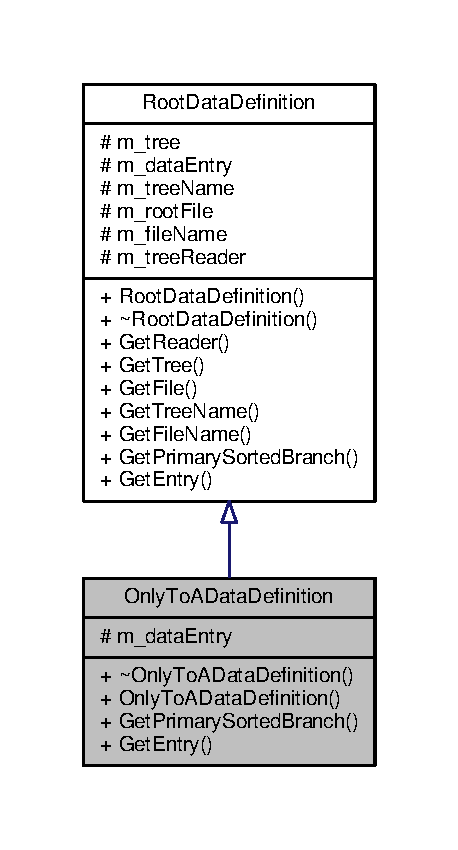
\includegraphics[width=220pt]{classOnlyToADataDefinition__inherit__graph}
\end{center}
\end{figure}


Collaboration diagram for Only\+To\+A\+Data\+Definition\+:\nopagebreak
\begin{figure}[H]
\begin{center}
\leavevmode
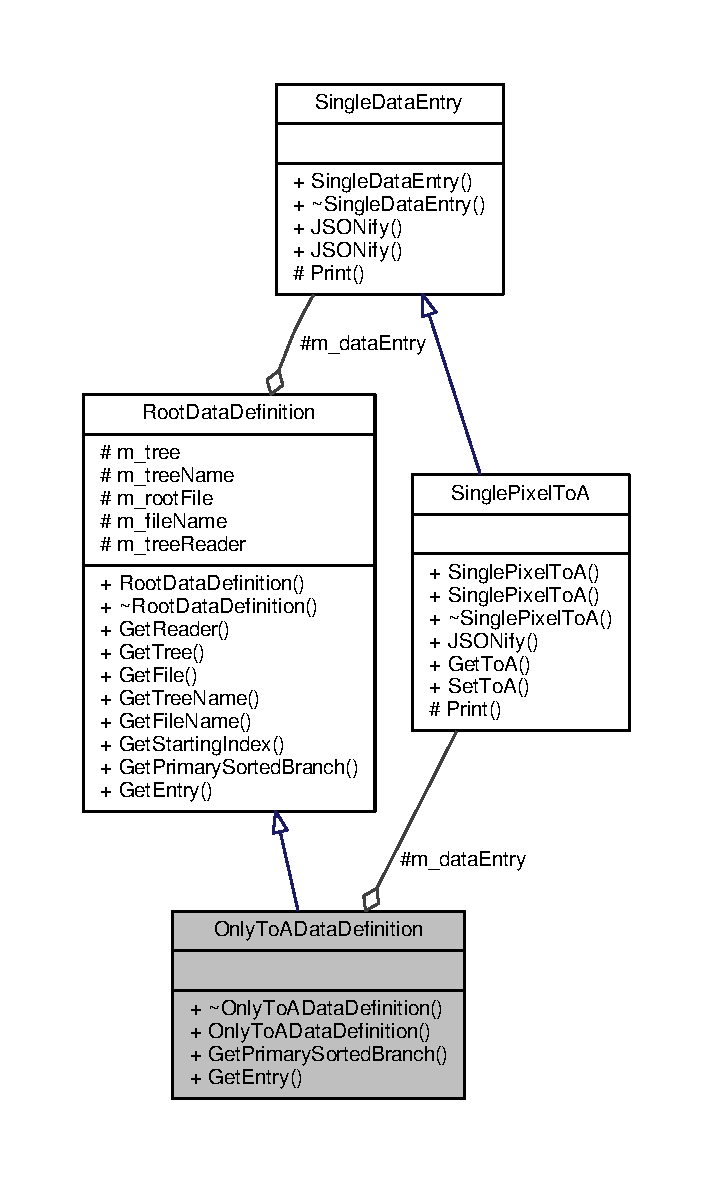
\includegraphics[height=550pt]{classOnlyToADataDefinition__coll__graph}
\end{center}
\end{figure}
\subsection*{Public Member Functions}
\begin{DoxyCompactItemize}
\item 
\hyperlink{classOnlyToADataDefinition_ac3392db2f04c84cfce35bbf12f287357}{$\sim$\+Only\+To\+A\+Data\+Definition} ()
\item 
\hyperlink{classOnlyToADataDefinition_aee47039c5d1c4c8714815e0253fca3e3}{Only\+To\+A\+Data\+Definition} (std\+::string file\+Name, std\+::string tree\+Name)
\item 
void $\ast$ \hyperlink{classOnlyToADataDefinition_af2025f39b59dc8bd50a281f5034ed47a}{Get\+Primary\+Sorted\+Branch} ()
\item 
\hyperlink{classSingleDataEntry}{Single\+Data\+Entry} $\ast$ \hyperlink{classOnlyToADataDefinition_ab2f4346c01cf342390c392cf1e36eebe}{Get\+Entry} ()
\end{DoxyCompactItemize}
\subsection*{Protected Attributes}
\begin{DoxyCompactItemize}
\item 
\hyperlink{classSinglePixelToA}{Single\+Pixel\+To\+A} $\ast$ \hyperlink{classOnlyToADataDefinition_abb0a23c47fcf037c042e8529163a1e31}{m\+\_\+data\+Entry} = new \hyperlink{classSinglePixelToA}{Single\+Pixel\+To\+A}()
\end{DoxyCompactItemize}


\subsection{Detailed Description}
Class defining the structure of data within root file containing only one value (of type double) -\/ To\+A. 

\subsection{Constructor \& Destructor Documentation}
\hypertarget{classOnlyToADataDefinition_ac3392db2f04c84cfce35bbf12f287357}{\index{Only\+To\+A\+Data\+Definition@{Only\+To\+A\+Data\+Definition}!````~Only\+To\+A\+Data\+Definition@{$\sim$\+Only\+To\+A\+Data\+Definition}}
\index{````~Only\+To\+A\+Data\+Definition@{$\sim$\+Only\+To\+A\+Data\+Definition}!Only\+To\+A\+Data\+Definition@{Only\+To\+A\+Data\+Definition}}
\subsubsection[{$\sim$\+Only\+To\+A\+Data\+Definition}]{\setlength{\rightskip}{0pt plus 5cm}Only\+To\+A\+Data\+Definition\+::$\sim$\+Only\+To\+A\+Data\+Definition (
\begin{DoxyParamCaption}
{}
\end{DoxyParamCaption}
)}}\label{classOnlyToADataDefinition_ac3392db2f04c84cfce35bbf12f287357}
\hypertarget{classOnlyToADataDefinition_aee47039c5d1c4c8714815e0253fca3e3}{\index{Only\+To\+A\+Data\+Definition@{Only\+To\+A\+Data\+Definition}!Only\+To\+A\+Data\+Definition@{Only\+To\+A\+Data\+Definition}}
\index{Only\+To\+A\+Data\+Definition@{Only\+To\+A\+Data\+Definition}!Only\+To\+A\+Data\+Definition@{Only\+To\+A\+Data\+Definition}}
\subsubsection[{Only\+To\+A\+Data\+Definition}]{\setlength{\rightskip}{0pt plus 5cm}Only\+To\+A\+Data\+Definition\+::\+Only\+To\+A\+Data\+Definition (
\begin{DoxyParamCaption}
\item[{std\+::string}]{file\+Name, }
\item[{std\+::string}]{tree\+Name}
\end{DoxyParamCaption}
)}}\label{classOnlyToADataDefinition_aee47039c5d1c4c8714815e0253fca3e3}


\subsection{Member Function Documentation}
\hypertarget{classOnlyToADataDefinition_ab2f4346c01cf342390c392cf1e36eebe}{\index{Only\+To\+A\+Data\+Definition@{Only\+To\+A\+Data\+Definition}!Get\+Entry@{Get\+Entry}}
\index{Get\+Entry@{Get\+Entry}!Only\+To\+A\+Data\+Definition@{Only\+To\+A\+Data\+Definition}}
\subsubsection[{Get\+Entry}]{\setlength{\rightskip}{0pt plus 5cm}{\bf Single\+Data\+Entry} $\ast$ Only\+To\+A\+Data\+Definition\+::\+Get\+Entry (
\begin{DoxyParamCaption}
{}
\end{DoxyParamCaption}
)\hspace{0.3cm}{\ttfamily [virtual]}}}\label{classOnlyToADataDefinition_ab2f4346c01cf342390c392cf1e36eebe}


Implements \hyperlink{classRootDataDefinition_a60bb9c8884bdaca62fa342bfa6cf0bdb}{Root\+Data\+Definition}.

\hypertarget{classOnlyToADataDefinition_af2025f39b59dc8bd50a281f5034ed47a}{\index{Only\+To\+A\+Data\+Definition@{Only\+To\+A\+Data\+Definition}!Get\+Primary\+Sorted\+Branch@{Get\+Primary\+Sorted\+Branch}}
\index{Get\+Primary\+Sorted\+Branch@{Get\+Primary\+Sorted\+Branch}!Only\+To\+A\+Data\+Definition@{Only\+To\+A\+Data\+Definition}}
\subsubsection[{Get\+Primary\+Sorted\+Branch}]{\setlength{\rightskip}{0pt plus 5cm}void $\ast$ Only\+To\+A\+Data\+Definition\+::\+Get\+Primary\+Sorted\+Branch (
\begin{DoxyParamCaption}
{}
\end{DoxyParamCaption}
)\hspace{0.3cm}{\ttfamily [virtual]}}}\label{classOnlyToADataDefinition_af2025f39b59dc8bd50a281f5034ed47a}


Implements \hyperlink{classRootDataDefinition_a720d0b9c122b778f2b338792de9e8c47}{Root\+Data\+Definition}.



\subsection{Member Data Documentation}
\hypertarget{classOnlyToADataDefinition_abb0a23c47fcf037c042e8529163a1e31}{\index{Only\+To\+A\+Data\+Definition@{Only\+To\+A\+Data\+Definition}!m\+\_\+data\+Entry@{m\+\_\+data\+Entry}}
\index{m\+\_\+data\+Entry@{m\+\_\+data\+Entry}!Only\+To\+A\+Data\+Definition@{Only\+To\+A\+Data\+Definition}}
\subsubsection[{m\+\_\+data\+Entry}]{\setlength{\rightskip}{0pt plus 5cm}{\bf Single\+Pixel\+To\+A}$\ast$ Only\+To\+A\+Data\+Definition\+::m\+\_\+data\+Entry = new {\bf Single\+Pixel\+To\+A}()\hspace{0.3cm}{\ttfamily [protected]}}}\label{classOnlyToADataDefinition_abb0a23c47fcf037c042e8529163a1e31}


The documentation for this class was generated from the following files\+:\begin{DoxyCompactItemize}
\item 
src/\hyperlink{OnlyToADataDefinition_8h}{Only\+To\+A\+Data\+Definition.\+h}\item 
src/\hyperlink{OnlyToADataDefinition_8cpp}{Only\+To\+A\+Data\+Definition.\+cpp}\end{DoxyCompactItemize}

\hypertarget{classRootDataDefinition}{\section{Root\+Data\+Definition Class Reference}
\label{classRootDataDefinition}\index{Root\+Data\+Definition@{Root\+Data\+Definition}}
}


Abstract interface for defining a structure of the data in the R\+O\+O\+T files, process how to read these data and save them to desired data objects.  




{\ttfamily \#include $<$Root\+Data\+Definition.\+h$>$}



Inheritance diagram for Root\+Data\+Definition\+:\nopagebreak
\begin{figure}[H]
\begin{center}
\leavevmode
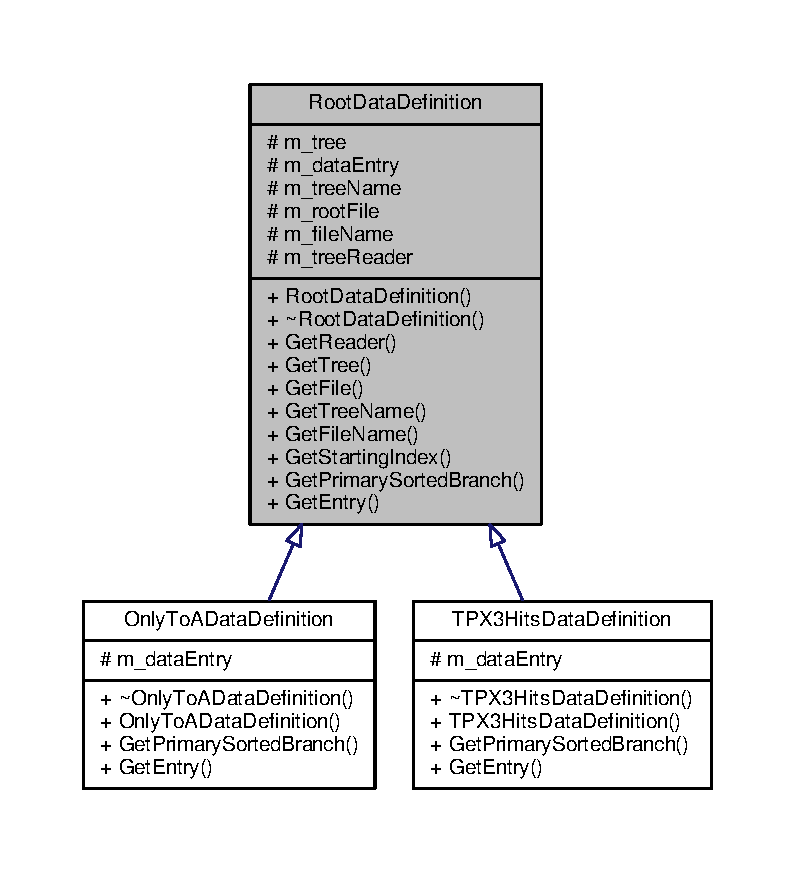
\includegraphics[width=220pt]{classRootDataDefinition__inherit__graph}
\end{center}
\end{figure}


Collaboration diagram for Root\+Data\+Definition\+:\nopagebreak
\begin{figure}[H]
\begin{center}
\leavevmode
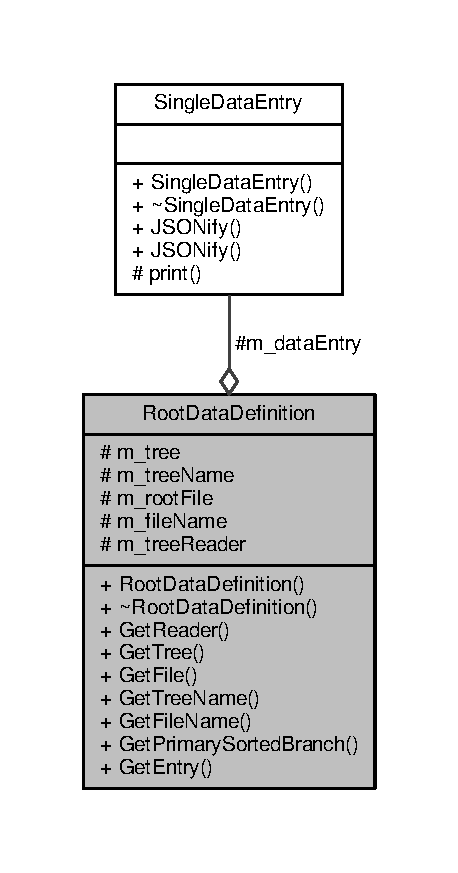
\includegraphics[width=220pt]{classRootDataDefinition__coll__graph}
\end{center}
\end{figure}
\subsection*{Public Member Functions}
\begin{DoxyCompactItemize}
\item 
\hyperlink{classRootDataDefinition_aeb304a3a15314058d6663c45c7f8f00e}{Root\+Data\+Definition} (std\+::string file\+Name, std\+::string tree\+Name)
\item 
virtual \hyperlink{classRootDataDefinition_a40a873fba464bcb796a444db890385dc}{$\sim$\+Root\+Data\+Definition} ()
\item 
T\+Tree\+Reader $\ast$ \hyperlink{classRootDataDefinition_a48a885b44c954506728f71f07d927506}{Get\+Reader} ()
\item 
T\+Tree $\ast$ \hyperlink{classRootDataDefinition_a20ed89d6d2483a0f76cd2fb131fcc597}{Get\+Tree} ()
\item 
T\+File $\ast$ \hyperlink{classRootDataDefinition_ab26897ffdd1de5e6572f6067770066b3}{Get\+File} ()
\item 
std\+::string \hyperlink{classRootDataDefinition_acc7728b0a9315cacc6b9c1fae38ed490}{Get\+Tree\+Name} ()
\item 
std\+::string \hyperlink{classRootDataDefinition_a56f206839275fdf5af290b372c4d7e13}{Get\+File\+Name} ()
\item 
virtual void $\ast$ \hyperlink{classRootDataDefinition_a720d0b9c122b778f2b338792de9e8c47}{Get\+Primary\+Sorted\+Branch} ()=0
\item 
virtual \hyperlink{classSingleDataEntry}{Single\+Data\+Entry} $\ast$ \hyperlink{classRootDataDefinition_a60bb9c8884bdaca62fa342bfa6cf0bdb}{Get\+Entry} ()=0
\end{DoxyCompactItemize}
\subsection*{Protected Attributes}
\begin{DoxyCompactItemize}
\item 
T\+Tree $\ast$ \hyperlink{classRootDataDefinition_a941ec585a2aa533bc30889a382e54f50}{m\+\_\+tree}
\item 
\hyperlink{classSingleDataEntry}{Single\+Data\+Entry} $\ast$ \hyperlink{classRootDataDefinition_a4d36dedf6212d7096b0020e9c1be9247}{m\+\_\+data\+Entry}
\item 
std\+::string \hyperlink{classRootDataDefinition_a46394bbb1863baa4abcd8cbd0413fa88}{m\+\_\+tree\+Name}
\item 
T\+File $\ast$ \hyperlink{classRootDataDefinition_af00a892a1b940abf9265066391b67304}{m\+\_\+root\+File}
\item 
std\+::string \hyperlink{classRootDataDefinition_a03154139db8613ec02cd57fd84d8c0e8}{m\+\_\+file\+Name}
\item 
T\+Tree\+Reader $\ast$ \hyperlink{classRootDataDefinition_a919827bdd245e61c0f54676d59cc7448}{m\+\_\+tree\+Reader}
\end{DoxyCompactItemize}


\subsection{Detailed Description}
Abstract interface for defining a structure of the data in the R\+O\+O\+T files, process how to read these data and save them to desired data objects. 

All data structure definitions have to derive from this interface and have to contain methods described by it.

Defines\+:
\begin{DoxyItemize}
\item which R\+O\+O\+T file, tree and branches are used.
\item which data to read from the R\+O\+O\+T tree
\item which data object (derived from \hyperlink{classSingleDataEntry}{Single\+Data\+Entry}) will be used to represent and store these data
\item how to get values of the data object (\hyperlink{classSingleDataEntry}{Single\+Data\+Entry}) from the values in the R\+O\+O\+T tree and its branches 
\end{DoxyItemize}

Definition at line 20 of file Root\+Data\+Definition.\+h.



\subsection{Constructor \& Destructor Documentation}
\hypertarget{classRootDataDefinition_aeb304a3a15314058d6663c45c7f8f00e}{\index{Root\+Data\+Definition@{Root\+Data\+Definition}!Root\+Data\+Definition@{Root\+Data\+Definition}}
\index{Root\+Data\+Definition@{Root\+Data\+Definition}!Root\+Data\+Definition@{Root\+Data\+Definition}}
\subsubsection[{Root\+Data\+Definition}]{\setlength{\rightskip}{0pt plus 5cm}Root\+Data\+Definition\+::\+Root\+Data\+Definition (
\begin{DoxyParamCaption}
\item[{std\+::string}]{file\+Name, }
\item[{std\+::string}]{tree\+Name}
\end{DoxyParamCaption}
)}}\label{classRootDataDefinition_aeb304a3a15314058d6663c45c7f8f00e}


Definition at line 26 of file Root\+Data\+Definition.\+cpp.

\hypertarget{classRootDataDefinition_a40a873fba464bcb796a444db890385dc}{\index{Root\+Data\+Definition@{Root\+Data\+Definition}!````~Root\+Data\+Definition@{$\sim$\+Root\+Data\+Definition}}
\index{````~Root\+Data\+Definition@{$\sim$\+Root\+Data\+Definition}!Root\+Data\+Definition@{Root\+Data\+Definition}}
\subsubsection[{$\sim$\+Root\+Data\+Definition}]{\setlength{\rightskip}{0pt plus 5cm}virtual Root\+Data\+Definition\+::$\sim$\+Root\+Data\+Definition (
\begin{DoxyParamCaption}
{}
\end{DoxyParamCaption}
)\hspace{0.3cm}{\ttfamily [inline]}, {\ttfamily [virtual]}}}\label{classRootDataDefinition_a40a873fba464bcb796a444db890385dc}


Definition at line 30 of file Root\+Data\+Definition.\+h.



\subsection{Member Function Documentation}
\hypertarget{classRootDataDefinition_a60bb9c8884bdaca62fa342bfa6cf0bdb}{\index{Root\+Data\+Definition@{Root\+Data\+Definition}!Get\+Entry@{Get\+Entry}}
\index{Get\+Entry@{Get\+Entry}!Root\+Data\+Definition@{Root\+Data\+Definition}}
\subsubsection[{Get\+Entry}]{\setlength{\rightskip}{0pt plus 5cm}virtual {\bf Single\+Data\+Entry}$\ast$ Root\+Data\+Definition\+::\+Get\+Entry (
\begin{DoxyParamCaption}
{}
\end{DoxyParamCaption}
)\hspace{0.3cm}{\ttfamily [pure virtual]}}}\label{classRootDataDefinition_a60bb9c8884bdaca62fa342bfa6cf0bdb}


Implemented in \hyperlink{classOnlyToADataDefinition_ab2f4346c01cf342390c392cf1e36eebe}{Only\+To\+A\+Data\+Definition}.

\hypertarget{classRootDataDefinition_ab26897ffdd1de5e6572f6067770066b3}{\index{Root\+Data\+Definition@{Root\+Data\+Definition}!Get\+File@{Get\+File}}
\index{Get\+File@{Get\+File}!Root\+Data\+Definition@{Root\+Data\+Definition}}
\subsubsection[{Get\+File}]{\setlength{\rightskip}{0pt plus 5cm}T\+File $\ast$ Root\+Data\+Definition\+::\+Get\+File (
\begin{DoxyParamCaption}
{}
\end{DoxyParamCaption}
)}}\label{classRootDataDefinition_ab26897ffdd1de5e6572f6067770066b3}


Definition at line 14 of file Root\+Data\+Definition.\+cpp.

\hypertarget{classRootDataDefinition_a56f206839275fdf5af290b372c4d7e13}{\index{Root\+Data\+Definition@{Root\+Data\+Definition}!Get\+File\+Name@{Get\+File\+Name}}
\index{Get\+File\+Name@{Get\+File\+Name}!Root\+Data\+Definition@{Root\+Data\+Definition}}
\subsubsection[{Get\+File\+Name}]{\setlength{\rightskip}{0pt plus 5cm}std\+::string Root\+Data\+Definition\+::\+Get\+File\+Name (
\begin{DoxyParamCaption}
{}
\end{DoxyParamCaption}
)}}\label{classRootDataDefinition_a56f206839275fdf5af290b372c4d7e13}


Definition at line 22 of file Root\+Data\+Definition.\+cpp.

\hypertarget{classRootDataDefinition_a720d0b9c122b778f2b338792de9e8c47}{\index{Root\+Data\+Definition@{Root\+Data\+Definition}!Get\+Primary\+Sorted\+Branch@{Get\+Primary\+Sorted\+Branch}}
\index{Get\+Primary\+Sorted\+Branch@{Get\+Primary\+Sorted\+Branch}!Root\+Data\+Definition@{Root\+Data\+Definition}}
\subsubsection[{Get\+Primary\+Sorted\+Branch}]{\setlength{\rightskip}{0pt plus 5cm}virtual void$\ast$ Root\+Data\+Definition\+::\+Get\+Primary\+Sorted\+Branch (
\begin{DoxyParamCaption}
{}
\end{DoxyParamCaption}
)\hspace{0.3cm}{\ttfamily [pure virtual]}}}\label{classRootDataDefinition_a720d0b9c122b778f2b338792de9e8c47}


Implemented in \hyperlink{classOnlyToADataDefinition_af2025f39b59dc8bd50a281f5034ed47a}{Only\+To\+A\+Data\+Definition}.

\hypertarget{classRootDataDefinition_a48a885b44c954506728f71f07d927506}{\index{Root\+Data\+Definition@{Root\+Data\+Definition}!Get\+Reader@{Get\+Reader}}
\index{Get\+Reader@{Get\+Reader}!Root\+Data\+Definition@{Root\+Data\+Definition}}
\subsubsection[{Get\+Reader}]{\setlength{\rightskip}{0pt plus 5cm}T\+Tree\+Reader $\ast$ Root\+Data\+Definition\+::\+Get\+Reader (
\begin{DoxyParamCaption}
{}
\end{DoxyParamCaption}
)}}\label{classRootDataDefinition_a48a885b44c954506728f71f07d927506}


Definition at line 3 of file Root\+Data\+Definition.\+cpp.

\hypertarget{classRootDataDefinition_a20ed89d6d2483a0f76cd2fb131fcc597}{\index{Root\+Data\+Definition@{Root\+Data\+Definition}!Get\+Tree@{Get\+Tree}}
\index{Get\+Tree@{Get\+Tree}!Root\+Data\+Definition@{Root\+Data\+Definition}}
\subsubsection[{Get\+Tree}]{\setlength{\rightskip}{0pt plus 5cm}T\+Tree $\ast$ Root\+Data\+Definition\+::\+Get\+Tree (
\begin{DoxyParamCaption}
{}
\end{DoxyParamCaption}
)}}\label{classRootDataDefinition_a20ed89d6d2483a0f76cd2fb131fcc597}


Definition at line 7 of file Root\+Data\+Definition.\+cpp.

\hypertarget{classRootDataDefinition_acc7728b0a9315cacc6b9c1fae38ed490}{\index{Root\+Data\+Definition@{Root\+Data\+Definition}!Get\+Tree\+Name@{Get\+Tree\+Name}}
\index{Get\+Tree\+Name@{Get\+Tree\+Name}!Root\+Data\+Definition@{Root\+Data\+Definition}}
\subsubsection[{Get\+Tree\+Name}]{\setlength{\rightskip}{0pt plus 5cm}std\+::string Root\+Data\+Definition\+::\+Get\+Tree\+Name (
\begin{DoxyParamCaption}
{}
\end{DoxyParamCaption}
)}}\label{classRootDataDefinition_acc7728b0a9315cacc6b9c1fae38ed490}


Definition at line 18 of file Root\+Data\+Definition.\+cpp.



\subsection{Member Data Documentation}
\hypertarget{classRootDataDefinition_a4d36dedf6212d7096b0020e9c1be9247}{\index{Root\+Data\+Definition@{Root\+Data\+Definition}!m\+\_\+data\+Entry@{m\+\_\+data\+Entry}}
\index{m\+\_\+data\+Entry@{m\+\_\+data\+Entry}!Root\+Data\+Definition@{Root\+Data\+Definition}}
\subsubsection[{m\+\_\+data\+Entry}]{\setlength{\rightskip}{0pt plus 5cm}{\bf Single\+Data\+Entry}$\ast$ Root\+Data\+Definition\+::m\+\_\+data\+Entry\hspace{0.3cm}{\ttfamily [protected]}}}\label{classRootDataDefinition_a4d36dedf6212d7096b0020e9c1be9247}


Definition at line 23 of file Root\+Data\+Definition.\+h.

\hypertarget{classRootDataDefinition_a03154139db8613ec02cd57fd84d8c0e8}{\index{Root\+Data\+Definition@{Root\+Data\+Definition}!m\+\_\+file\+Name@{m\+\_\+file\+Name}}
\index{m\+\_\+file\+Name@{m\+\_\+file\+Name}!Root\+Data\+Definition@{Root\+Data\+Definition}}
\subsubsection[{m\+\_\+file\+Name}]{\setlength{\rightskip}{0pt plus 5cm}std\+::string Root\+Data\+Definition\+::m\+\_\+file\+Name\hspace{0.3cm}{\ttfamily [protected]}}}\label{classRootDataDefinition_a03154139db8613ec02cd57fd84d8c0e8}


Definition at line 26 of file Root\+Data\+Definition.\+h.

\hypertarget{classRootDataDefinition_af00a892a1b940abf9265066391b67304}{\index{Root\+Data\+Definition@{Root\+Data\+Definition}!m\+\_\+root\+File@{m\+\_\+root\+File}}
\index{m\+\_\+root\+File@{m\+\_\+root\+File}!Root\+Data\+Definition@{Root\+Data\+Definition}}
\subsubsection[{m\+\_\+root\+File}]{\setlength{\rightskip}{0pt plus 5cm}T\+File$\ast$ Root\+Data\+Definition\+::m\+\_\+root\+File\hspace{0.3cm}{\ttfamily [protected]}}}\label{classRootDataDefinition_af00a892a1b940abf9265066391b67304}


Definition at line 25 of file Root\+Data\+Definition.\+h.

\hypertarget{classRootDataDefinition_a941ec585a2aa533bc30889a382e54f50}{\index{Root\+Data\+Definition@{Root\+Data\+Definition}!m\+\_\+tree@{m\+\_\+tree}}
\index{m\+\_\+tree@{m\+\_\+tree}!Root\+Data\+Definition@{Root\+Data\+Definition}}
\subsubsection[{m\+\_\+tree}]{\setlength{\rightskip}{0pt plus 5cm}T\+Tree$\ast$ Root\+Data\+Definition\+::m\+\_\+tree\hspace{0.3cm}{\ttfamily [protected]}}}\label{classRootDataDefinition_a941ec585a2aa533bc30889a382e54f50}


Definition at line 22 of file Root\+Data\+Definition.\+h.

\hypertarget{classRootDataDefinition_a46394bbb1863baa4abcd8cbd0413fa88}{\index{Root\+Data\+Definition@{Root\+Data\+Definition}!m\+\_\+tree\+Name@{m\+\_\+tree\+Name}}
\index{m\+\_\+tree\+Name@{m\+\_\+tree\+Name}!Root\+Data\+Definition@{Root\+Data\+Definition}}
\subsubsection[{m\+\_\+tree\+Name}]{\setlength{\rightskip}{0pt plus 5cm}std\+::string Root\+Data\+Definition\+::m\+\_\+tree\+Name\hspace{0.3cm}{\ttfamily [protected]}}}\label{classRootDataDefinition_a46394bbb1863baa4abcd8cbd0413fa88}


Definition at line 24 of file Root\+Data\+Definition.\+h.

\hypertarget{classRootDataDefinition_a919827bdd245e61c0f54676d59cc7448}{\index{Root\+Data\+Definition@{Root\+Data\+Definition}!m\+\_\+tree\+Reader@{m\+\_\+tree\+Reader}}
\index{m\+\_\+tree\+Reader@{m\+\_\+tree\+Reader}!Root\+Data\+Definition@{Root\+Data\+Definition}}
\subsubsection[{m\+\_\+tree\+Reader}]{\setlength{\rightskip}{0pt plus 5cm}T\+Tree\+Reader$\ast$ Root\+Data\+Definition\+::m\+\_\+tree\+Reader\hspace{0.3cm}{\ttfamily [protected]}}}\label{classRootDataDefinition_a919827bdd245e61c0f54676d59cc7448}


Definition at line 27 of file Root\+Data\+Definition.\+h.



The documentation for this class was generated from the following files\+:\begin{DoxyCompactItemize}
\item 
src/\hyperlink{RootDataDefinition_8h}{Root\+Data\+Definition.\+h}\item 
src/\hyperlink{RootDataDefinition_8cpp}{Root\+Data\+Definition.\+cpp}\end{DoxyCompactItemize}

\hypertarget{classRootDataReader}{\section{Root\+Data\+Reader Class Reference}
\label{classRootDataReader}\index{Root\+Data\+Reader@{Root\+Data\+Reader}}
}


Class responsible for reading data of various structure in the R\+O\+O\+T format (T\+Tree within T\+File).  




{\ttfamily \#include $<$Root\+Data\+Reader.\+h$>$}



Collaboration diagram for Root\+Data\+Reader\+:\nopagebreak
\begin{figure}[H]
\begin{center}
\leavevmode
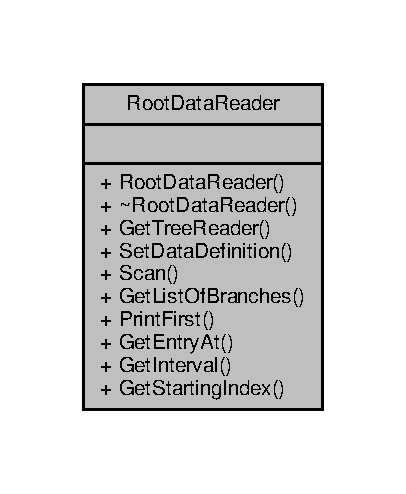
\includegraphics[width=191pt]{classRootDataReader__coll__graph}
\end{center}
\end{figure}
\subsection*{Public Member Functions}
\begin{DoxyCompactItemize}
\item 
\hyperlink{classRootDataReader_aa06f1264959329cb49e41a7670e6a59f}{Root\+Data\+Reader} ()
\item 
\hyperlink{classRootDataReader_a9f6b5d9e26e27128a445ac3529414f6f}{$\sim$\+Root\+Data\+Reader} ()
\item 
T\+Tree\+Reader $\ast$ \hyperlink{classRootDataReader_a749a090b6c0404f9ff08873a2aef63d7}{Get\+Tree\+Reader} ()
\item 
void \hyperlink{classRootDataReader_ad670745df69f90ea6578d7c29cab716f}{Set\+Data\+Definition} (\hyperlink{classRootDataDefinition}{Root\+Data\+Definition} $\ast$definition)
\item 
void \hyperlink{classRootDataReader_a22eac63f0710d5cce4a1d0a16210ce8f}{Scan} ()
\item 
bool \hyperlink{classRootDataReader_aac09b1313c7ce2c180b5efede781eef6}{Print\+First} ()
\item 
\hyperlink{classSingleDataEntry}{Single\+Data\+Entry} $\ast$ \hyperlink{classRootDataReader_abd5fbaefe8631cf251e9aeade874fa5d}{Get\+Entry\+At} (unsigned int index)
\item 
\hyperlink{classDataEntryInterval}{Data\+Entry\+Interval} $\ast$ \hyperlink{classRootDataReader_a76a02dd2cc6f4cde896ce9180048671b}{Get\+Interval} (unsigned int index\+From, unsigned int index\+To)
\end{DoxyCompactItemize}


\subsection{Detailed Description}
Class responsible for reading data of various structure in the R\+O\+O\+T format (T\+Tree within T\+File). 

\hyperlink{classRootDataReader}{Root\+Data\+Reader} provides a facade for accessing arbitrary data from R\+O\+O\+T files, providing them in C++ custom interval class, standard C++ vector or a J\+S\+O\+N format.

After setting the proper \hyperlink{classRootDataDefinition}{Root\+Data\+Definition}, \hyperlink{classRootDataReader}{Root\+Data\+Reader} will know the structure of the data it will be working with. Then it can read data of such structure and retrieve them as a whole, as a std\+::vector, as a interval, print them to stdout etc. 

Definition at line 13 of file Root\+Data\+Reader.\+h.



\subsection{Constructor \& Destructor Documentation}
\hypertarget{classRootDataReader_aa06f1264959329cb49e41a7670e6a59f}{\index{Root\+Data\+Reader@{Root\+Data\+Reader}!Root\+Data\+Reader@{Root\+Data\+Reader}}
\index{Root\+Data\+Reader@{Root\+Data\+Reader}!Root\+Data\+Reader@{Root\+Data\+Reader}}
\subsubsection[{Root\+Data\+Reader}]{\setlength{\rightskip}{0pt plus 5cm}Root\+Data\+Reader\+::\+Root\+Data\+Reader (
\begin{DoxyParamCaption}
{}
\end{DoxyParamCaption}
)}}\label{classRootDataReader_aa06f1264959329cb49e41a7670e6a59f}


Definition at line 3 of file Root\+Data\+Reader.\+cpp.

\hypertarget{classRootDataReader_a9f6b5d9e26e27128a445ac3529414f6f}{\index{Root\+Data\+Reader@{Root\+Data\+Reader}!````~Root\+Data\+Reader@{$\sim$\+Root\+Data\+Reader}}
\index{````~Root\+Data\+Reader@{$\sim$\+Root\+Data\+Reader}!Root\+Data\+Reader@{Root\+Data\+Reader}}
\subsubsection[{$\sim$\+Root\+Data\+Reader}]{\setlength{\rightskip}{0pt plus 5cm}Root\+Data\+Reader\+::$\sim$\+Root\+Data\+Reader (
\begin{DoxyParamCaption}
{}
\end{DoxyParamCaption}
)}}\label{classRootDataReader_a9f6b5d9e26e27128a445ac3529414f6f}


Definition at line 8 of file Root\+Data\+Reader.\+cpp.



\subsection{Member Function Documentation}
\hypertarget{classRootDataReader_abd5fbaefe8631cf251e9aeade874fa5d}{\index{Root\+Data\+Reader@{Root\+Data\+Reader}!Get\+Entry\+At@{Get\+Entry\+At}}
\index{Get\+Entry\+At@{Get\+Entry\+At}!Root\+Data\+Reader@{Root\+Data\+Reader}}
\subsubsection[{Get\+Entry\+At}]{\setlength{\rightskip}{0pt plus 5cm}{\bf Single\+Data\+Entry} $\ast$ Root\+Data\+Reader\+::\+Get\+Entry\+At (
\begin{DoxyParamCaption}
\item[{unsigned int}]{index}
\end{DoxyParamCaption}
)}}\label{classRootDataReader_abd5fbaefe8631cf251e9aeade874fa5d}


Definition at line 32 of file Root\+Data\+Reader.\+cpp.

\hypertarget{classRootDataReader_a76a02dd2cc6f4cde896ce9180048671b}{\index{Root\+Data\+Reader@{Root\+Data\+Reader}!Get\+Interval@{Get\+Interval}}
\index{Get\+Interval@{Get\+Interval}!Root\+Data\+Reader@{Root\+Data\+Reader}}
\subsubsection[{Get\+Interval}]{\setlength{\rightskip}{0pt plus 5cm}{\bf Data\+Entry\+Interval} $\ast$ Root\+Data\+Reader\+::\+Get\+Interval (
\begin{DoxyParamCaption}
\item[{unsigned int}]{index\+From, }
\item[{unsigned int}]{index\+To}
\end{DoxyParamCaption}
)}}\label{classRootDataReader_a76a02dd2cc6f4cde896ce9180048671b}


Definition at line 40 of file Root\+Data\+Reader.\+cpp.

\hypertarget{classRootDataReader_a749a090b6c0404f9ff08873a2aef63d7}{\index{Root\+Data\+Reader@{Root\+Data\+Reader}!Get\+Tree\+Reader@{Get\+Tree\+Reader}}
\index{Get\+Tree\+Reader@{Get\+Tree\+Reader}!Root\+Data\+Reader@{Root\+Data\+Reader}}
\subsubsection[{Get\+Tree\+Reader}]{\setlength{\rightskip}{0pt plus 5cm}T\+Tree\+Reader $\ast$ Root\+Data\+Reader\+::\+Get\+Tree\+Reader (
\begin{DoxyParamCaption}
{}
\end{DoxyParamCaption}
)}}\label{classRootDataReader_a749a090b6c0404f9ff08873a2aef63d7}


Definition at line 55 of file Root\+Data\+Reader.\+cpp.

\hypertarget{classRootDataReader_aac09b1313c7ce2c180b5efede781eef6}{\index{Root\+Data\+Reader@{Root\+Data\+Reader}!Print\+First@{Print\+First}}
\index{Print\+First@{Print\+First}!Root\+Data\+Reader@{Root\+Data\+Reader}}
\subsubsection[{Print\+First}]{\setlength{\rightskip}{0pt plus 5cm}bool Root\+Data\+Reader\+::\+Print\+First (
\begin{DoxyParamCaption}
{}
\end{DoxyParamCaption}
)}}\label{classRootDataReader_aac09b1313c7ce2c180b5efede781eef6}
Prints the first entry in the specified T\+Tree within specified T\+File, according to specified \hyperlink{classRootDataDefinition}{Root\+Data\+Definition} \begin{DoxyReturn}{Returns}
true if success 

false if there was an error and printing couldn't happen 
\end{DoxyReturn}


Definition at line 23 of file Root\+Data\+Reader.\+cpp.

\hypertarget{classRootDataReader_a22eac63f0710d5cce4a1d0a16210ce8f}{\index{Root\+Data\+Reader@{Root\+Data\+Reader}!Scan@{Scan}}
\index{Scan@{Scan}!Root\+Data\+Reader@{Root\+Data\+Reader}}
\subsubsection[{Scan}]{\setlength{\rightskip}{0pt plus 5cm}void Root\+Data\+Reader\+::\+Scan (
\begin{DoxyParamCaption}
{}
\end{DoxyParamCaption}
)}}\label{classRootDataReader_a22eac63f0710d5cce4a1d0a16210ce8f}


Definition at line 19 of file Root\+Data\+Reader.\+cpp.

\hypertarget{classRootDataReader_ad670745df69f90ea6578d7c29cab716f}{\index{Root\+Data\+Reader@{Root\+Data\+Reader}!Set\+Data\+Definition@{Set\+Data\+Definition}}
\index{Set\+Data\+Definition@{Set\+Data\+Definition}!Root\+Data\+Reader@{Root\+Data\+Reader}}
\subsubsection[{Set\+Data\+Definition}]{\setlength{\rightskip}{0pt plus 5cm}void Root\+Data\+Reader\+::\+Set\+Data\+Definition (
\begin{DoxyParamCaption}
\item[{{\bf Root\+Data\+Definition} $\ast$}]{definition}
\end{DoxyParamCaption}
)}}\label{classRootDataReader_ad670745df69f90ea6578d7c29cab716f}


Definition at line 14 of file Root\+Data\+Reader.\+cpp.



The documentation for this class was generated from the following files\+:\begin{DoxyCompactItemize}
\item 
src/\hyperlink{RootDataReader_8h}{Root\+Data\+Reader.\+h}\item 
src/\hyperlink{RootDataReader_8cpp}{Root\+Data\+Reader.\+cpp}\end{DoxyCompactItemize}

\hypertarget{classSingleDataEntry}{\section{Single\+Data\+Entry Class Reference}
\label{classSingleDataEntry}\index{Single\+Data\+Entry@{Single\+Data\+Entry}}
}


Abstract class representing a data object to be retrieved from the R\+O\+O\+T file.  




{\ttfamily \#include $<$Single\+Data\+Entry.\+h$>$}



Inheritance diagram for Single\+Data\+Entry\+:
\nopagebreak
\begin{figure}[H]
\begin{center}
\leavevmode
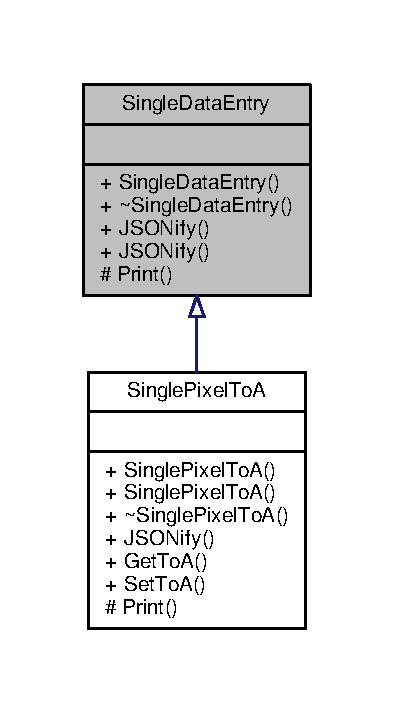
\includegraphics[width=304pt]{classSingleDataEntry__inherit__graph}
\end{center}
\end{figure}


Collaboration diagram for Single\+Data\+Entry\+:
\nopagebreak
\begin{figure}[H]
\begin{center}
\leavevmode
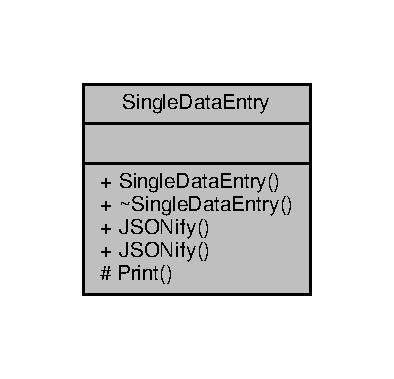
\includegraphics[width=189pt]{classSingleDataEntry__coll__graph}
\end{center}
\end{figure}
\subsection*{Public Member Functions}
\begin{DoxyCompactItemize}
\item 
\hyperlink{classSingleDataEntry_a64f6763312181cd57157bafe94f9a4ee}{Single\+Data\+Entry} ()
\begin{DoxyCompactList}\small\item\em Implicit base constructor, does nothing. \end{DoxyCompactList}\item 
virtual \hyperlink{classSingleDataEntry_a0b6b6ebca677d8cd87062db2f354f364}{$\sim$\+Single\+Data\+Entry} ()
\begin{DoxyCompactList}\small\item\em Virtual destructor. Each derived class has to dispose of their own garbage. \end{DoxyCompactList}\item 
virtual void \hyperlink{classSingleDataEntry_a64fb67b2f11f2fe64394059f1b29a248}{J\+S\+O\+Nify} (rapidjson\+::\+Writer$<$ rapidjson\+::\+String\+Buffer $>$ \&writer)=0
\begin{DoxyCompactList}\small\item\em Writes the J\+S\+O\+N representation of this one single entry into the specified J\+S\+O\+N writer. \end{DoxyCompactList}\item 
std\+::string \hyperlink{classSingleDataEntry_a9e48725016d6fbd6bd674d5b299dbb12}{J\+S\+O\+Nify} ()
\begin{DoxyCompactList}\small\item\em Returns J\+S\+O\+N string serialization of this object. \end{DoxyCompactList}\end{DoxyCompactItemize}
\subsection*{Protected Member Functions}
\begin{DoxyCompactItemize}
\item 
virtual void \hyperlink{classSingleDataEntry_a16006af8d5648c79ee9e6c6ed6c356a2}{Print} (std\+::ostream \&os) const =0
\begin{DoxyCompactList}\small\item\em Prints the data entry into specified stream. \end{DoxyCompactList}\end{DoxyCompactItemize}
\subsection*{Friends}
\begin{DoxyCompactItemize}
\item 
std\+::ostream \& \hyperlink{classSingleDataEntry_a5201741bff3d8419b28d56bda6a8dc2d}{operator$<$$<$} (std\+::ostream \&os, const \hyperlink{classSingleDataEntry}{Single\+Data\+Entry} \&entry)
\begin{DoxyCompactList}\small\item\em Prints the data entry using its print function. \end{DoxyCompactList}\end{DoxyCompactItemize}


\subsection{Detailed Description}
Abstract class representing a data object to be retrieved from the R\+O\+O\+T file. 

Represents the result object we want to work with after retrieving the data from R\+O\+O\+T files. Specifies the object's attributes and their types, way how to print them or serialize them. The whole object can be printed to a stream, can be serialized to J\+S\+O\+N. 

Definition at line 16 of file Single\+Data\+Entry.\+h.



\subsection{Constructor \& Destructor Documentation}
\hypertarget{classSingleDataEntry_a64f6763312181cd57157bafe94f9a4ee}{\index{Single\+Data\+Entry@{Single\+Data\+Entry}!Single\+Data\+Entry@{Single\+Data\+Entry}}
\index{Single\+Data\+Entry@{Single\+Data\+Entry}!Single\+Data\+Entry@{Single\+Data\+Entry}}
\subsubsection[{Single\+Data\+Entry}]{\setlength{\rightskip}{0pt plus 5cm}Single\+Data\+Entry\+::\+Single\+Data\+Entry (
\begin{DoxyParamCaption}
{}
\end{DoxyParamCaption}
)\hspace{0.3cm}{\ttfamily [inline]}}}\label{classSingleDataEntry_a64f6763312181cd57157bafe94f9a4ee}


Implicit base constructor, does nothing. 



Definition at line 24 of file Single\+Data\+Entry.\+h.

\hypertarget{classSingleDataEntry_a0b6b6ebca677d8cd87062db2f354f364}{\index{Single\+Data\+Entry@{Single\+Data\+Entry}!````~Single\+Data\+Entry@{$\sim$\+Single\+Data\+Entry}}
\index{````~Single\+Data\+Entry@{$\sim$\+Single\+Data\+Entry}!Single\+Data\+Entry@{Single\+Data\+Entry}}
\subsubsection[{$\sim$\+Single\+Data\+Entry}]{\setlength{\rightskip}{0pt plus 5cm}virtual Single\+Data\+Entry\+::$\sim$\+Single\+Data\+Entry (
\begin{DoxyParamCaption}
{}
\end{DoxyParamCaption}
)\hspace{0.3cm}{\ttfamily [inline]}, {\ttfamily [virtual]}}}\label{classSingleDataEntry_a0b6b6ebca677d8cd87062db2f354f364}


Virtual destructor. Each derived class has to dispose of their own garbage. 



Definition at line 26 of file Single\+Data\+Entry.\+h.



\subsection{Member Function Documentation}
\hypertarget{classSingleDataEntry_a64fb67b2f11f2fe64394059f1b29a248}{\index{Single\+Data\+Entry@{Single\+Data\+Entry}!J\+S\+O\+Nify@{J\+S\+O\+Nify}}
\index{J\+S\+O\+Nify@{J\+S\+O\+Nify}!Single\+Data\+Entry@{Single\+Data\+Entry}}
\subsubsection[{J\+S\+O\+Nify}]{\setlength{\rightskip}{0pt plus 5cm}virtual void Single\+Data\+Entry\+::\+J\+S\+O\+Nify (
\begin{DoxyParamCaption}
\item[{rapidjson\+::\+Writer$<$ rapidjson\+::\+String\+Buffer $>$ \&}]{writer}
\end{DoxyParamCaption}
)\hspace{0.3cm}{\ttfamily [pure virtual]}}}\label{classSingleDataEntry_a64fb67b2f11f2fe64394059f1b29a248}


Writes the J\+S\+O\+N representation of this one single entry into the specified J\+S\+O\+N writer. 



Implemented in \hyperlink{classSingleTPX3Hit_aaa523b209e9f72fce0c6f9ca0b565b17}{Single\+T\+P\+X3\+Hit}, and \hyperlink{classSinglePixelToA_afef10aa4fe0b3c4d1676ada1d8ee4195}{Single\+Pixel\+To\+A}.

\hypertarget{classSingleDataEntry_a9e48725016d6fbd6bd674d5b299dbb12}{\index{Single\+Data\+Entry@{Single\+Data\+Entry}!J\+S\+O\+Nify@{J\+S\+O\+Nify}}
\index{J\+S\+O\+Nify@{J\+S\+O\+Nify}!Single\+Data\+Entry@{Single\+Data\+Entry}}
\subsubsection[{J\+S\+O\+Nify}]{\setlength{\rightskip}{0pt plus 5cm}std\+::string Single\+Data\+Entry\+::\+J\+S\+O\+Nify (
\begin{DoxyParamCaption}
{}
\end{DoxyParamCaption}
)\hspace{0.3cm}{\ttfamily [inline]}}}\label{classSingleDataEntry_a9e48725016d6fbd6bd674d5b299dbb12}


Returns J\+S\+O\+N string serialization of this object. 



Definition at line 35 of file Single\+Data\+Entry.\+h.

\hypertarget{classSingleDataEntry_a16006af8d5648c79ee9e6c6ed6c356a2}{\index{Single\+Data\+Entry@{Single\+Data\+Entry}!Print@{Print}}
\index{Print@{Print}!Single\+Data\+Entry@{Single\+Data\+Entry}}
\subsubsection[{Print}]{\setlength{\rightskip}{0pt plus 5cm}virtual void Single\+Data\+Entry\+::\+Print (
\begin{DoxyParamCaption}
\item[{std\+::ostream \&}]{os}
\end{DoxyParamCaption}
) const\hspace{0.3cm}{\ttfamily [protected]}, {\ttfamily [pure virtual]}}}\label{classSingleDataEntry_a16006af8d5648c79ee9e6c6ed6c356a2}


Prints the data entry into specified stream. 



Implemented in \hyperlink{classSingleTPX3Hit_a552a56d164a8c0c02d06e56c1a367355}{Single\+T\+P\+X3\+Hit}, and \hyperlink{classSinglePixelToA_a8b9d4ef4082473c747157b9b2c1376b0}{Single\+Pixel\+To\+A}.



\subsection{Friends And Related Function Documentation}
\hypertarget{classSingleDataEntry_a5201741bff3d8419b28d56bda6a8dc2d}{\index{Single\+Data\+Entry@{Single\+Data\+Entry}!operator$<$$<$@{operator$<$$<$}}
\index{operator$<$$<$@{operator$<$$<$}!Single\+Data\+Entry@{Single\+Data\+Entry}}
\subsubsection[{operator$<$$<$}]{\setlength{\rightskip}{0pt plus 5cm}std\+::ostream\& operator$<$$<$ (
\begin{DoxyParamCaption}
\item[{std\+::ostream \&}]{os, }
\item[{const {\bf Single\+Data\+Entry} \&}]{entry}
\end{DoxyParamCaption}
)\hspace{0.3cm}{\ttfamily [friend]}}}\label{classSingleDataEntry_a5201741bff3d8419b28d56bda6a8dc2d}


Prints the data entry using its print function. 



Definition at line 28 of file Single\+Data\+Entry.\+h.



The documentation for this class was generated from the following file\+:\begin{DoxyCompactItemize}
\item 
src/\hyperlink{SingleDataEntry_8h}{Single\+Data\+Entry.\+h}\end{DoxyCompactItemize}

\hypertarget{classSinglePixelToA}{\section{Single\+Pixel\+To\+A Class Reference}
\label{classSinglePixelToA}\index{Single\+Pixel\+To\+A@{Single\+Pixel\+To\+A}}
}


Class defining the data object containing only single value (of type double) -\/ To\+A.  




{\ttfamily \#include $<$Single\+Pixel\+To\+A.\+h$>$}



Inheritance diagram for Single\+Pixel\+To\+A\+:
\nopagebreak
\begin{figure}[H]
\begin{center}
\leavevmode
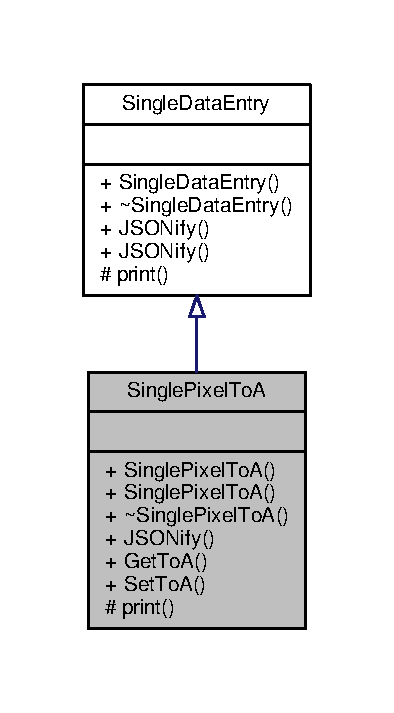
\includegraphics[width=189pt]{classSinglePixelToA__inherit__graph}
\end{center}
\end{figure}


Collaboration diagram for Single\+Pixel\+To\+A\+:
\nopagebreak
\begin{figure}[H]
\begin{center}
\leavevmode
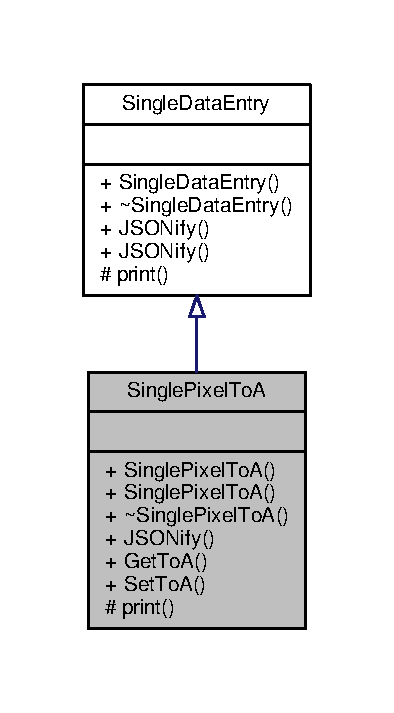
\includegraphics[width=189pt]{classSinglePixelToA__coll__graph}
\end{center}
\end{figure}
\subsection*{Public Member Functions}
\begin{DoxyCompactItemize}
\item 
\hyperlink{classSinglePixelToA_a14b5fa35ac80341c180ee2948b0d533a}{Single\+Pixel\+To\+A} ()
\begin{DoxyCompactList}\small\item\em Creates an empty pixel. \end{DoxyCompactList}\item 
\hyperlink{classSinglePixelToA_a848f55b6ef644f7b61a276aa0ec5c479}{Single\+Pixel\+To\+A} (\hyperlink{classSinglePixelToA}{Single\+Pixel\+To\+A} $\ast$other\+Pixel)
\begin{DoxyCompactList}\small\item\em Copy constructor. \end{DoxyCompactList}\item 
\hyperlink{classSinglePixelToA_a976faa699430463edccf827d7686f941}{$\sim$\+Single\+Pixel\+To\+A} ()
\begin{DoxyCompactList}\small\item\em Implicit destructor. \end{DoxyCompactList}\item 
void \hyperlink{classSinglePixelToA_afef10aa4fe0b3c4d1676ada1d8ee4195}{J\+S\+O\+Nify} (rapidjson\+::\+Writer$<$ rapidjson\+::\+String\+Buffer $>$ \&writer)
\begin{DoxyCompactList}\small\item\em Writes the J\+S\+O\+N representation of this one single entry into the specified J\+S\+O\+N writer. \end{DoxyCompactList}\item 
Double\+\_\+t \hyperlink{classSinglePixelToA_ac63323a38df82131599539bf412e5c4e}{Get\+To\+A} () const 
\item 
void \hyperlink{classSinglePixelToA_a7c3836057703bd042c89997e3490d3d9}{Set\+To\+A} (Double\+\_\+t To\+A)
\item 
std\+::string \hyperlink{classSingleDataEntry_a9e48725016d6fbd6bd674d5b299dbb12}{J\+S\+O\+Nify} ()
\begin{DoxyCompactList}\small\item\em Returns J\+S\+O\+N string serialization of this object. \end{DoxyCompactList}\end{DoxyCompactItemize}
\subsection*{Protected Member Functions}
\begin{DoxyCompactItemize}
\item 
void \hyperlink{classSinglePixelToA_a8b9d4ef4082473c747157b9b2c1376b0}{Print} (std\+::ostream \&os) const 
\begin{DoxyCompactList}\small\item\em Prints the data entry into specified stream. \end{DoxyCompactList}\end{DoxyCompactItemize}


\subsection{Detailed Description}
Class defining the data object containing only single value (of type double) -\/ To\+A. 

Definition at line 8 of file Single\+Pixel\+To\+A.\+h.



\subsection{Constructor \& Destructor Documentation}
\hypertarget{classSinglePixelToA_a14b5fa35ac80341c180ee2948b0d533a}{\index{Single\+Pixel\+To\+A@{Single\+Pixel\+To\+A}!Single\+Pixel\+To\+A@{Single\+Pixel\+To\+A}}
\index{Single\+Pixel\+To\+A@{Single\+Pixel\+To\+A}!Single\+Pixel\+To\+A@{Single\+Pixel\+To\+A}}
\subsubsection[{Single\+Pixel\+To\+A}]{\setlength{\rightskip}{0pt plus 5cm}Single\+Pixel\+To\+A\+::\+Single\+Pixel\+To\+A (
\begin{DoxyParamCaption}
{}
\end{DoxyParamCaption}
)}}\label{classSinglePixelToA_a14b5fa35ac80341c180ee2948b0d533a}


Creates an empty pixel. 



Definition at line 5 of file Single\+Pixel\+To\+A.\+cpp.

\hypertarget{classSinglePixelToA_a848f55b6ef644f7b61a276aa0ec5c479}{\index{Single\+Pixel\+To\+A@{Single\+Pixel\+To\+A}!Single\+Pixel\+To\+A@{Single\+Pixel\+To\+A}}
\index{Single\+Pixel\+To\+A@{Single\+Pixel\+To\+A}!Single\+Pixel\+To\+A@{Single\+Pixel\+To\+A}}
\subsubsection[{Single\+Pixel\+To\+A}]{\setlength{\rightskip}{0pt plus 5cm}Single\+Pixel\+To\+A\+::\+Single\+Pixel\+To\+A (
\begin{DoxyParamCaption}
\item[{{\bf Single\+Pixel\+To\+A} $\ast$}]{other\+Pixel}
\end{DoxyParamCaption}
)}}\label{classSinglePixelToA_a848f55b6ef644f7b61a276aa0ec5c479}


Copy constructor. 



Definition at line 9 of file Single\+Pixel\+To\+A.\+cpp.

\hypertarget{classSinglePixelToA_a976faa699430463edccf827d7686f941}{\index{Single\+Pixel\+To\+A@{Single\+Pixel\+To\+A}!````~Single\+Pixel\+To\+A@{$\sim$\+Single\+Pixel\+To\+A}}
\index{````~Single\+Pixel\+To\+A@{$\sim$\+Single\+Pixel\+To\+A}!Single\+Pixel\+To\+A@{Single\+Pixel\+To\+A}}
\subsubsection[{$\sim$\+Single\+Pixel\+To\+A}]{\setlength{\rightskip}{0pt plus 5cm}Single\+Pixel\+To\+A\+::$\sim$\+Single\+Pixel\+To\+A (
\begin{DoxyParamCaption}
{}
\end{DoxyParamCaption}
)}}\label{classSinglePixelToA_a976faa699430463edccf827d7686f941}


Implicit destructor. 



Definition at line 13 of file Single\+Pixel\+To\+A.\+cpp.



\subsection{Member Function Documentation}
\hypertarget{classSinglePixelToA_ac63323a38df82131599539bf412e5c4e}{\index{Single\+Pixel\+To\+A@{Single\+Pixel\+To\+A}!Get\+To\+A@{Get\+To\+A}}
\index{Get\+To\+A@{Get\+To\+A}!Single\+Pixel\+To\+A@{Single\+Pixel\+To\+A}}
\subsubsection[{Get\+To\+A}]{\setlength{\rightskip}{0pt plus 5cm}Double\+\_\+t Single\+Pixel\+To\+A\+::\+Get\+To\+A (
\begin{DoxyParamCaption}
{}
\end{DoxyParamCaption}
) const}}\label{classSinglePixelToA_ac63323a38df82131599539bf412e5c4e}


Definition at line 28 of file Single\+Pixel\+To\+A.\+cpp.

\hypertarget{classSinglePixelToA_afef10aa4fe0b3c4d1676ada1d8ee4195}{\index{Single\+Pixel\+To\+A@{Single\+Pixel\+To\+A}!J\+S\+O\+Nify@{J\+S\+O\+Nify}}
\index{J\+S\+O\+Nify@{J\+S\+O\+Nify}!Single\+Pixel\+To\+A@{Single\+Pixel\+To\+A}}
\subsubsection[{J\+S\+O\+Nify}]{\setlength{\rightskip}{0pt plus 5cm}void Single\+Pixel\+To\+A\+::\+J\+S\+O\+Nify (
\begin{DoxyParamCaption}
\item[{rapidjson\+::\+Writer$<$ rapidjson\+::\+String\+Buffer $>$ \&}]{writer}
\end{DoxyParamCaption}
)\hspace{0.3cm}{\ttfamily [virtual]}}}\label{classSinglePixelToA_afef10aa4fe0b3c4d1676ada1d8ee4195}


Writes the J\+S\+O\+N representation of this one single entry into the specified J\+S\+O\+N writer. 



Implements \hyperlink{classSingleDataEntry_a64fb67b2f11f2fe64394059f1b29a248}{Single\+Data\+Entry}.



Definition at line 21 of file Single\+Pixel\+To\+A.\+cpp.

\hypertarget{classSingleDataEntry_a9e48725016d6fbd6bd674d5b299dbb12}{\index{Single\+Pixel\+To\+A@{Single\+Pixel\+To\+A}!J\+S\+O\+Nify@{J\+S\+O\+Nify}}
\index{J\+S\+O\+Nify@{J\+S\+O\+Nify}!Single\+Pixel\+To\+A@{Single\+Pixel\+To\+A}}
\subsubsection[{J\+S\+O\+Nify}]{\setlength{\rightskip}{0pt plus 5cm}std\+::string Single\+Data\+Entry\+::\+J\+S\+O\+Nify (
\begin{DoxyParamCaption}
{}
\end{DoxyParamCaption}
)\hspace{0.3cm}{\ttfamily [inline]}, {\ttfamily [inherited]}}}\label{classSingleDataEntry_a9e48725016d6fbd6bd674d5b299dbb12}


Returns J\+S\+O\+N string serialization of this object. 



Definition at line 35 of file Single\+Data\+Entry.\+h.

\hypertarget{classSinglePixelToA_a8b9d4ef4082473c747157b9b2c1376b0}{\index{Single\+Pixel\+To\+A@{Single\+Pixel\+To\+A}!Print@{Print}}
\index{Print@{Print}!Single\+Pixel\+To\+A@{Single\+Pixel\+To\+A}}
\subsubsection[{Print}]{\setlength{\rightskip}{0pt plus 5cm}void Single\+Pixel\+To\+A\+::\+Print (
\begin{DoxyParamCaption}
\item[{std\+::ostream \&}]{os}
\end{DoxyParamCaption}
) const\hspace{0.3cm}{\ttfamily [protected]}, {\ttfamily [virtual]}}}\label{classSinglePixelToA_a8b9d4ef4082473c747157b9b2c1376b0}


Prints the data entry into specified stream. 



Implements \hyperlink{classSingleDataEntry_a16006af8d5648c79ee9e6c6ed6c356a2}{Single\+Data\+Entry}.



Definition at line 17 of file Single\+Pixel\+To\+A.\+cpp.

\hypertarget{classSinglePixelToA_a7c3836057703bd042c89997e3490d3d9}{\index{Single\+Pixel\+To\+A@{Single\+Pixel\+To\+A}!Set\+To\+A@{Set\+To\+A}}
\index{Set\+To\+A@{Set\+To\+A}!Single\+Pixel\+To\+A@{Single\+Pixel\+To\+A}}
\subsubsection[{Set\+To\+A}]{\setlength{\rightskip}{0pt plus 5cm}void Single\+Pixel\+To\+A\+::\+Set\+To\+A (
\begin{DoxyParamCaption}
\item[{Double\+\_\+t}]{To\+A}
\end{DoxyParamCaption}
)}}\label{classSinglePixelToA_a7c3836057703bd042c89997e3490d3d9}


Definition at line 32 of file Single\+Pixel\+To\+A.\+cpp.



The documentation for this class was generated from the following files\+:\begin{DoxyCompactItemize}
\item 
src/\hyperlink{SinglePixelToA_8h}{Single\+Pixel\+To\+A.\+h}\item 
src/\hyperlink{SinglePixelToA_8cpp}{Single\+Pixel\+To\+A.\+cpp}\end{DoxyCompactItemize}

\chapter{File Documentation}
\hypertarget{README_8md}{\section{R\+E\+A\+D\+M\+E.\+md File Reference}
\label{README_8md}\index{R\+E\+A\+D\+M\+E.\+md@{R\+E\+A\+D\+M\+E.\+md}}
}

\hypertarget{DataEntryInterval_8cpp}{\section{src/\+Data\+Entry\+Interval.cpp File Reference}
\label{DataEntryInterval_8cpp}\index{src/\+Data\+Entry\+Interval.\+cpp@{src/\+Data\+Entry\+Interval.\+cpp}}
}
{\ttfamily \#include \char`\"{}Data\+Entry\+Interval.\+h\char`\"{}}\\*
Include dependency graph for Data\+Entry\+Interval.\+cpp\+:\nopagebreak
\begin{figure}[H]
\begin{center}
\leavevmode
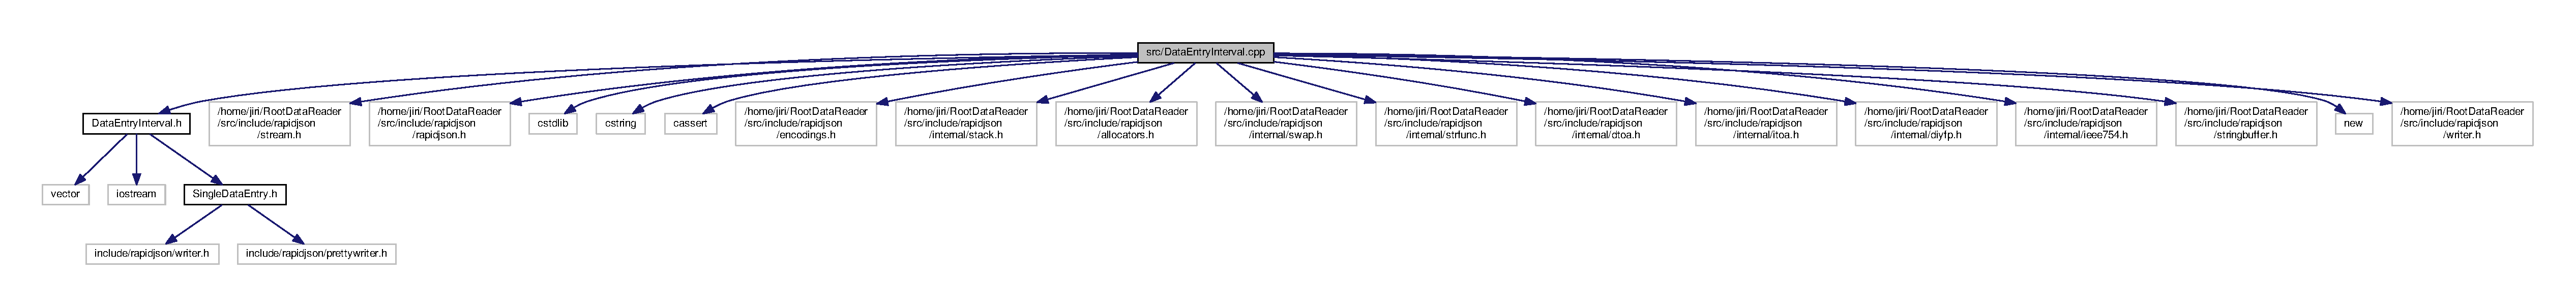
\includegraphics[width=350pt]{DataEntryInterval_8cpp__incl}
\end{center}
\end{figure}

\hypertarget{DataEntryInterval_8h}{\section{src/\+Data\+Entry\+Interval.h File Reference}
\label{DataEntryInterval_8h}\index{src/\+Data\+Entry\+Interval.\+h@{src/\+Data\+Entry\+Interval.\+h}}
}
{\ttfamily \#include $<$vector$>$}\\*
{\ttfamily \#include $<$iostream$>$}\\*
{\ttfamily \#include \char`\"{}Single\+Data\+Entry.\+h\char`\"{}}\\*
Include dependency graph for Data\+Entry\+Interval.\+h\+:
\nopagebreak
\begin{figure}[H]
\begin{center}
\leavevmode
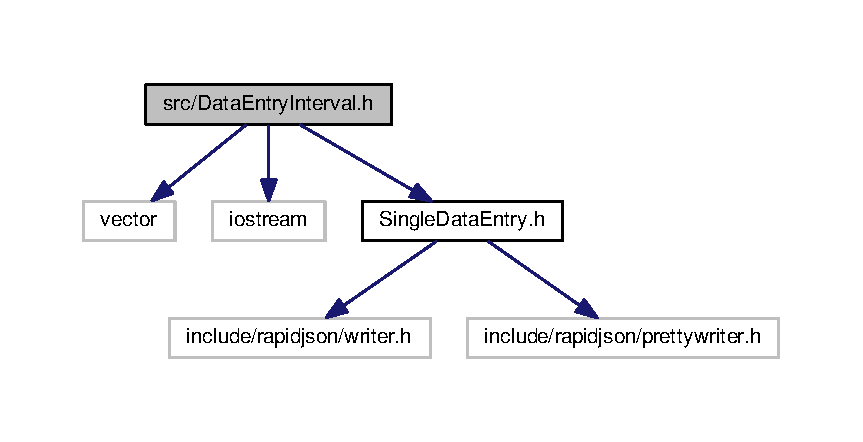
\includegraphics[width=350pt]{DataEntryInterval_8h__incl}
\end{center}
\end{figure}
This graph shows which files directly or indirectly include this file\+:
\nopagebreak
\begin{figure}[H]
\begin{center}
\leavevmode
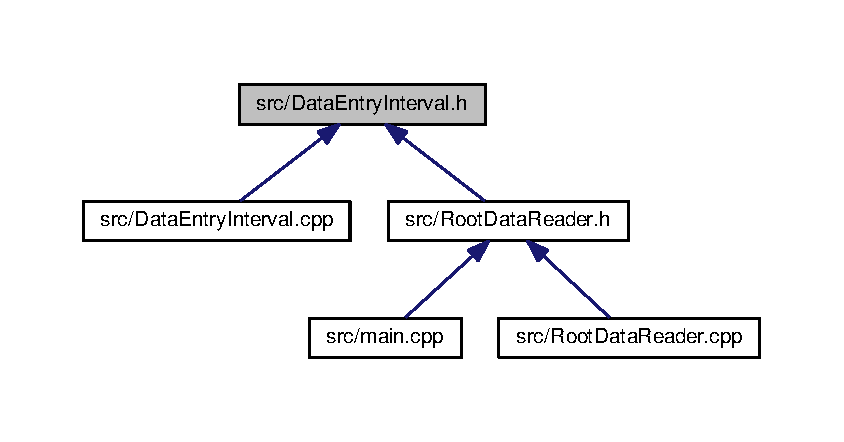
\includegraphics[width=350pt]{DataEntryInterval_8h__dep__incl}
\end{center}
\end{figure}
\subsection*{Classes}
\begin{DoxyCompactItemize}
\item 
class \hyperlink{classDataEntryInterval}{Data\+Entry\+Interval}
\begin{DoxyCompactList}\small\item\em The class representing an interval of root data entries. \end{DoxyCompactList}\end{DoxyCompactItemize}

\hypertarget{main_8cpp}{\section{src/main.cpp File Reference}
\label{main_8cpp}\index{src/main.\+cpp@{src/main.\+cpp}}
}
{\ttfamily \#include \char`\"{}Root\+Data\+Reader.\+h\char`\"{}}\\*
{\ttfamily \#include \char`\"{}Only\+To\+A\+Data\+Definition.\+h\char`\"{}}\\*
{\ttfamily \#include $<$typeinfo$>$}\\*
{\ttfamily \#include $<$iostream$>$}\\*
{\ttfamily \#include $<$unistd.\+h$>$}\\*
Include dependency graph for main.\+cpp\+:\nopagebreak
\begin{figure}[H]
\begin{center}
\leavevmode
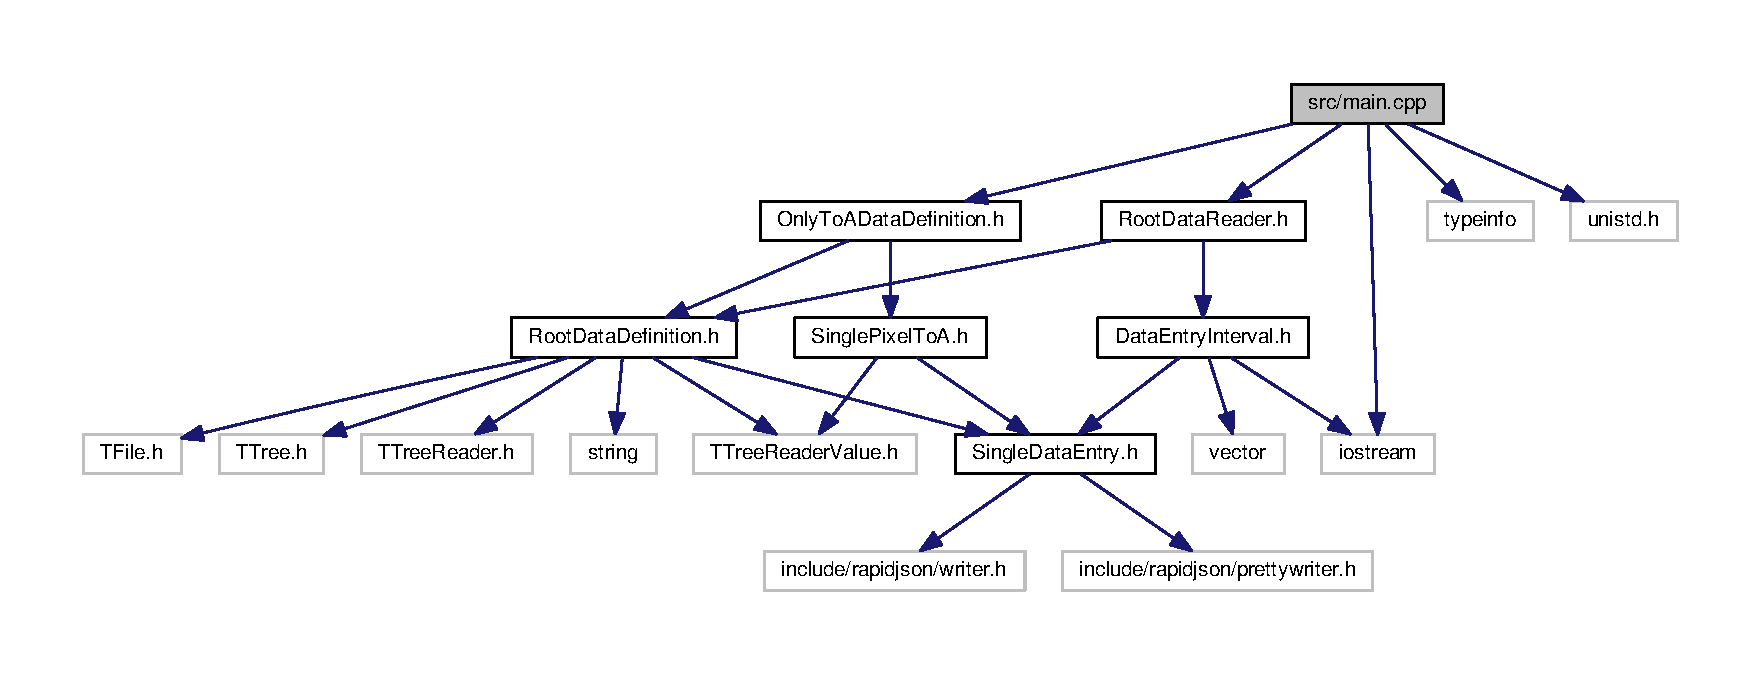
\includegraphics[width=350pt]{main_8cpp__incl}
\end{center}
\end{figure}
\subsection*{Functions}
\begin{DoxyCompactItemize}
\item 
int \hyperlink{main_8cpp_a840291bc02cba5474a4cb46a9b9566fe}{main} (void)
\end{DoxyCompactItemize}


\subsection{Function Documentation}
\hypertarget{main_8cpp_a840291bc02cba5474a4cb46a9b9566fe}{\index{main.\+cpp@{main.\+cpp}!main@{main}}
\index{main@{main}!main.\+cpp@{main.\+cpp}}
\subsubsection[{main}]{\setlength{\rightskip}{0pt plus 5cm}int main (
\begin{DoxyParamCaption}
\item[{void}]{}
\end{DoxyParamCaption}
)}}\label{main_8cpp_a840291bc02cba5474a4cb46a9b9566fe}


Definition at line 10 of file main.\+cpp.


\hypertarget{OnlyToADataDefinition_8cpp}{\section{src/\+Only\+To\+A\+Data\+Definition.cpp File Reference}
\label{OnlyToADataDefinition_8cpp}\index{src/\+Only\+To\+A\+Data\+Definition.\+cpp@{src/\+Only\+To\+A\+Data\+Definition.\+cpp}}
}
{\ttfamily \#include \char`\"{}Only\+To\+A\+Data\+Definition.\+h\char`\"{}}\\*
{\ttfamily \#include $<$typeinfo$>$}\\*
Include dependency graph for Only\+To\+A\+Data\+Definition.\+cpp\+:
\nopagebreak
\begin{figure}[H]
\begin{center}
\leavevmode
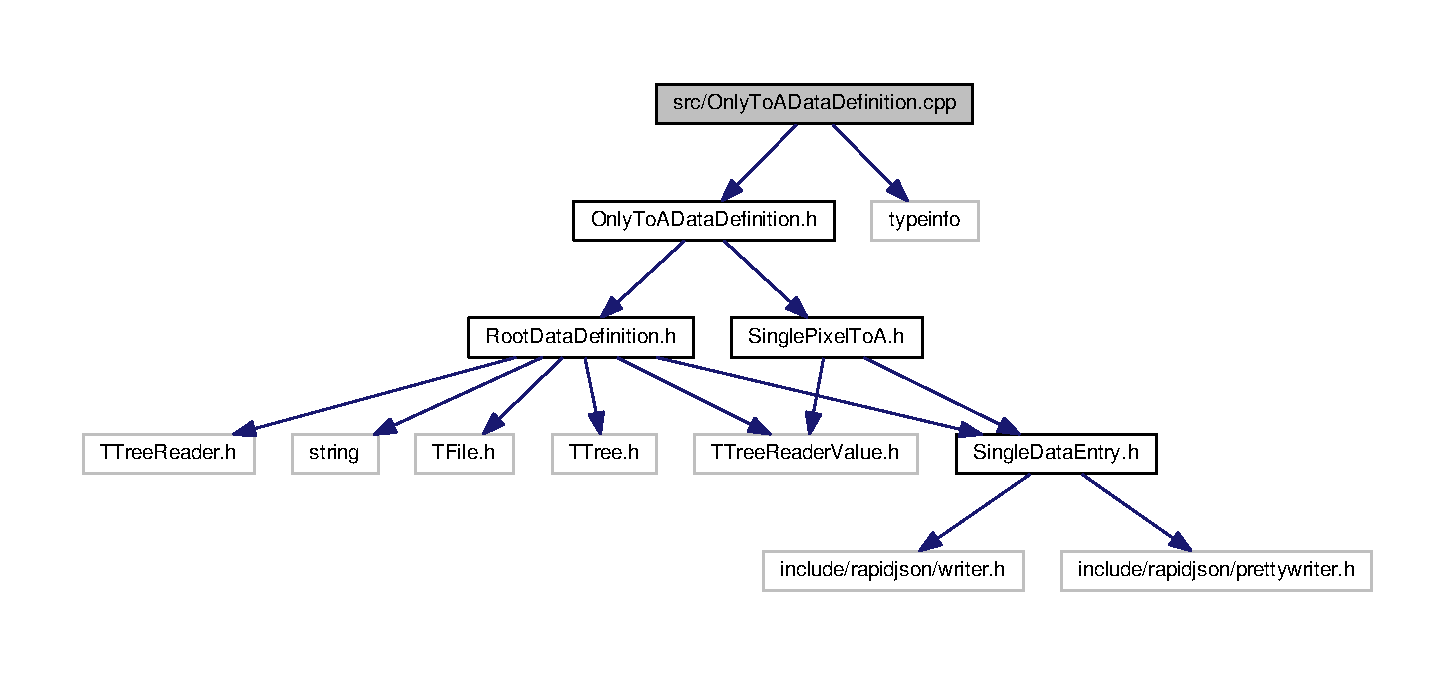
\includegraphics[width=350pt]{OnlyToADataDefinition_8cpp__incl}
\end{center}
\end{figure}

\hypertarget{OnlyToADataDefinition_8h}{\section{src/\+Only\+To\+A\+Data\+Definition.h File Reference}
\label{OnlyToADataDefinition_8h}\index{src/\+Only\+To\+A\+Data\+Definition.\+h@{src/\+Only\+To\+A\+Data\+Definition.\+h}}
}
{\ttfamily \#include \char`\"{}Root\+Data\+Definition.\+h\char`\"{}}\\*
{\ttfamily \#include \char`\"{}Single\+Pixel\+To\+A.\+h\char`\"{}}\\*
Include dependency graph for Only\+To\+A\+Data\+Definition.\+h\+:
\nopagebreak
\begin{figure}[H]
\begin{center}
\leavevmode
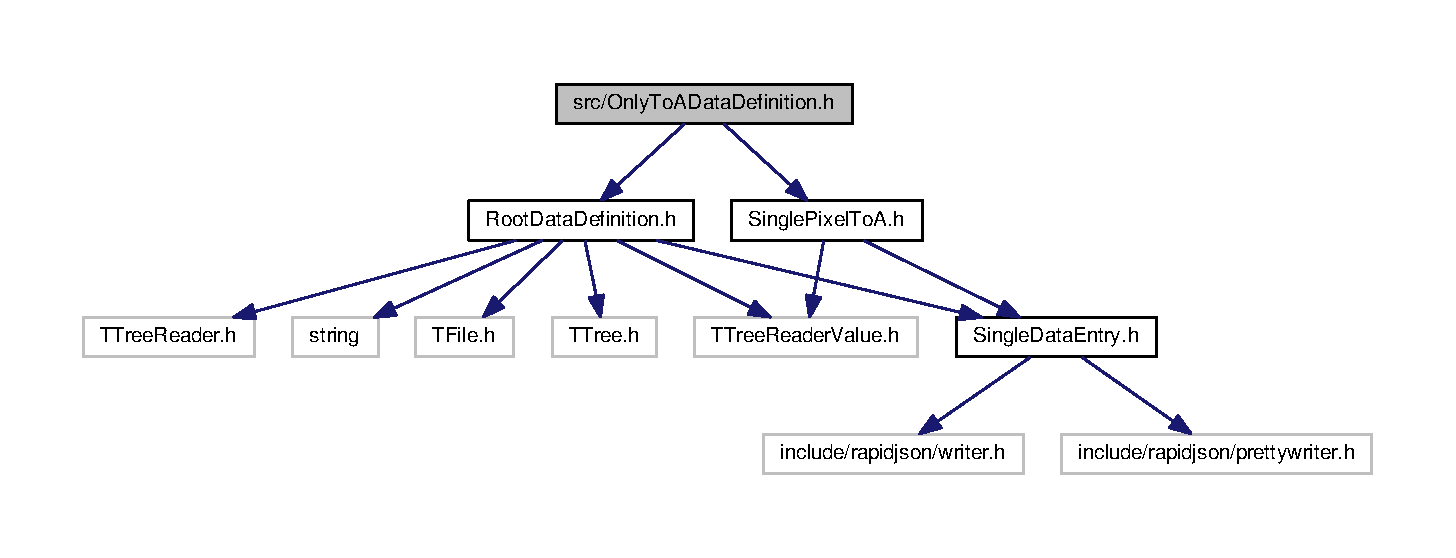
\includegraphics[width=350pt]{OnlyToADataDefinition_8h__incl}
\end{center}
\end{figure}
This graph shows which files directly or indirectly include this file\+:
\nopagebreak
\begin{figure}[H]
\begin{center}
\leavevmode
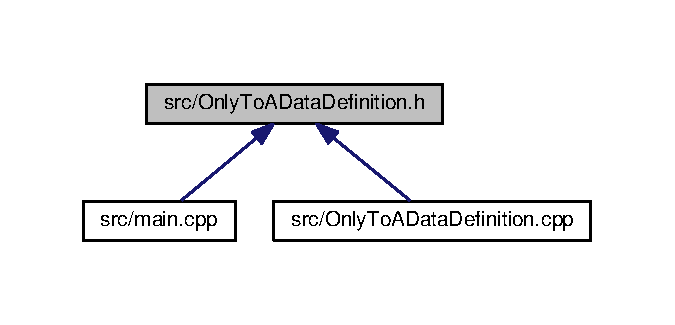
\includegraphics[width=324pt]{OnlyToADataDefinition_8h__dep__incl}
\end{center}
\end{figure}
\subsection*{Classes}
\begin{DoxyCompactItemize}
\item 
class \hyperlink{classOnlyToADataDefinition}{Only\+To\+A\+Data\+Definition}
\begin{DoxyCompactList}\small\item\em Class defining the structure of data within root file containing only one value (of type double) -\/ To\+A. \end{DoxyCompactList}\end{DoxyCompactItemize}

\hypertarget{RootDataDefinition_8cpp}{\section{src/\+Root\+Data\+Definition.cpp File Reference}
\label{RootDataDefinition_8cpp}\index{src/\+Root\+Data\+Definition.\+cpp@{src/\+Root\+Data\+Definition.\+cpp}}
}
{\ttfamily \#include \char`\"{}Root\+Data\+Definition.\+h\char`\"{}}\\*
Include dependency graph for Root\+Data\+Definition.\+cpp\+:\nopagebreak
\begin{figure}[H]
\begin{center}
\leavevmode
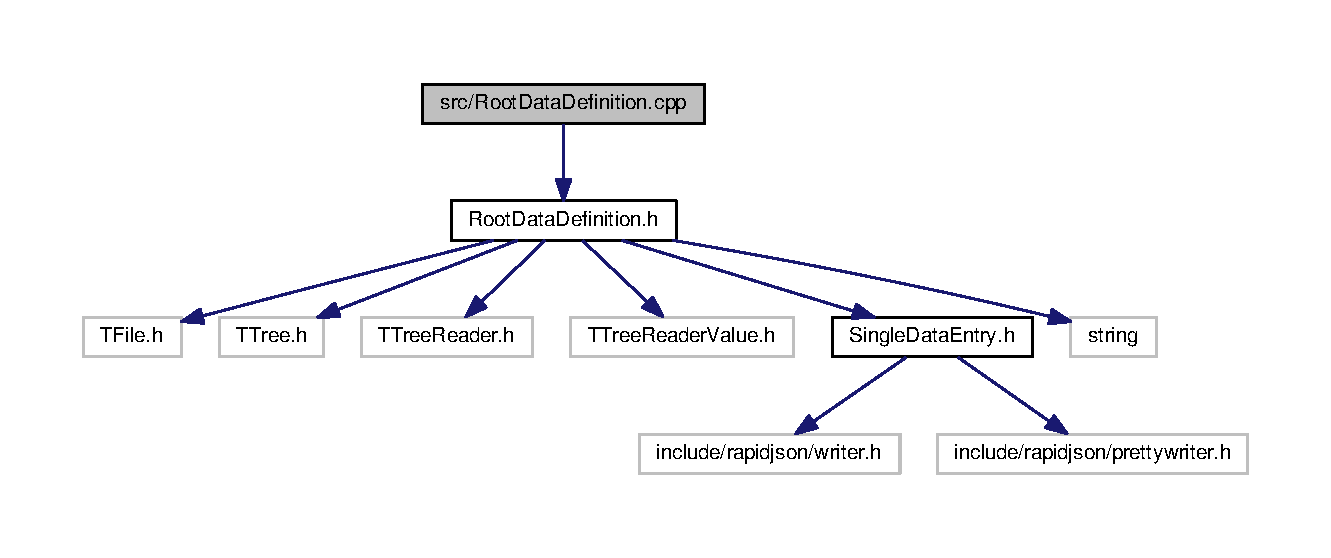
\includegraphics[width=350pt]{RootDataDefinition_8cpp__incl}
\end{center}
\end{figure}

\hypertarget{RootDataDefinition_8h}{\section{src/\+Root\+Data\+Definition.h File Reference}
\label{RootDataDefinition_8h}\index{src/\+Root\+Data\+Definition.\+h@{src/\+Root\+Data\+Definition.\+h}}
}
{\ttfamily \#include \char`\"{}T\+File.\+h\char`\"{}}\\*
{\ttfamily \#include \char`\"{}T\+Tree.\+h\char`\"{}}\\*
{\ttfamily \#include \char`\"{}T\+Tree\+Reader.\+h\char`\"{}}\\*
{\ttfamily \#include \char`\"{}T\+Tree\+Reader\+Value.\+h\char`\"{}}\\*
{\ttfamily \#include \char`\"{}Single\+Data\+Entry.\+h\char`\"{}}\\*
{\ttfamily \#include $<$string$>$}\\*
Include dependency graph for Root\+Data\+Definition.\+h\+:\nopagebreak
\begin{figure}[H]
\begin{center}
\leavevmode
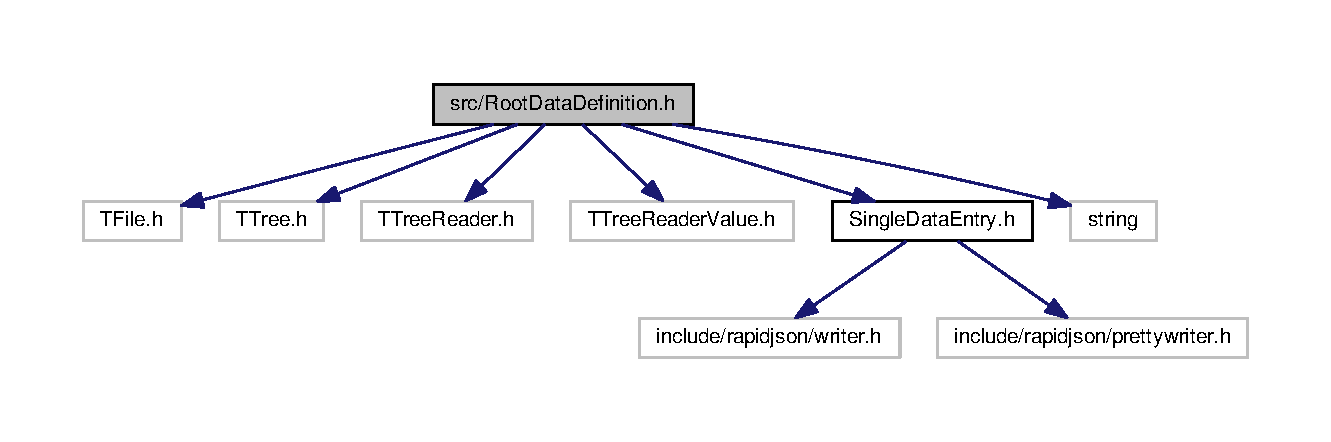
\includegraphics[width=350pt]{RootDataDefinition_8h__incl}
\end{center}
\end{figure}
This graph shows which files directly or indirectly include this file\+:\nopagebreak
\begin{figure}[H]
\begin{center}
\leavevmode
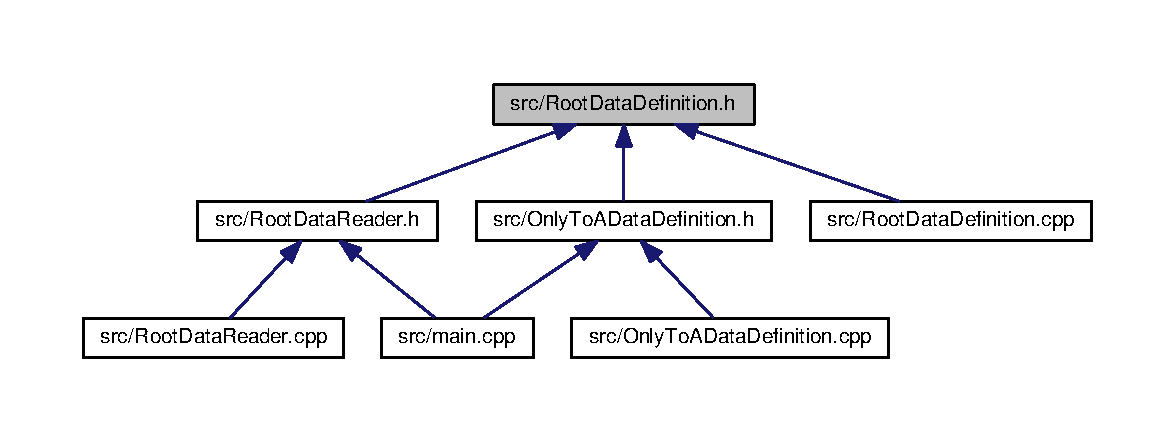
\includegraphics[width=350pt]{RootDataDefinition_8h__dep__incl}
\end{center}
\end{figure}
\subsection*{Classes}
\begin{DoxyCompactItemize}
\item 
class \hyperlink{classRootDataDefinition}{Root\+Data\+Definition}
\begin{DoxyCompactList}\small\item\em Abstract interface for defining a structure of the data in the R\+O\+O\+T files, process how to read these data and save them to desired data objects. \end{DoxyCompactList}\end{DoxyCompactItemize}

\hypertarget{RootDataReader_8cpp}{\section{src/\+Root\+Data\+Reader.cpp File Reference}
\label{RootDataReader_8cpp}\index{src/\+Root\+Data\+Reader.\+cpp@{src/\+Root\+Data\+Reader.\+cpp}}
}
{\ttfamily \#include \char`\"{}Root\+Data\+Reader.\+h\char`\"{}}\\*
Include dependency graph for Root\+Data\+Reader.\+cpp\+:
\nopagebreak
\begin{figure}[H]
\begin{center}
\leavevmode
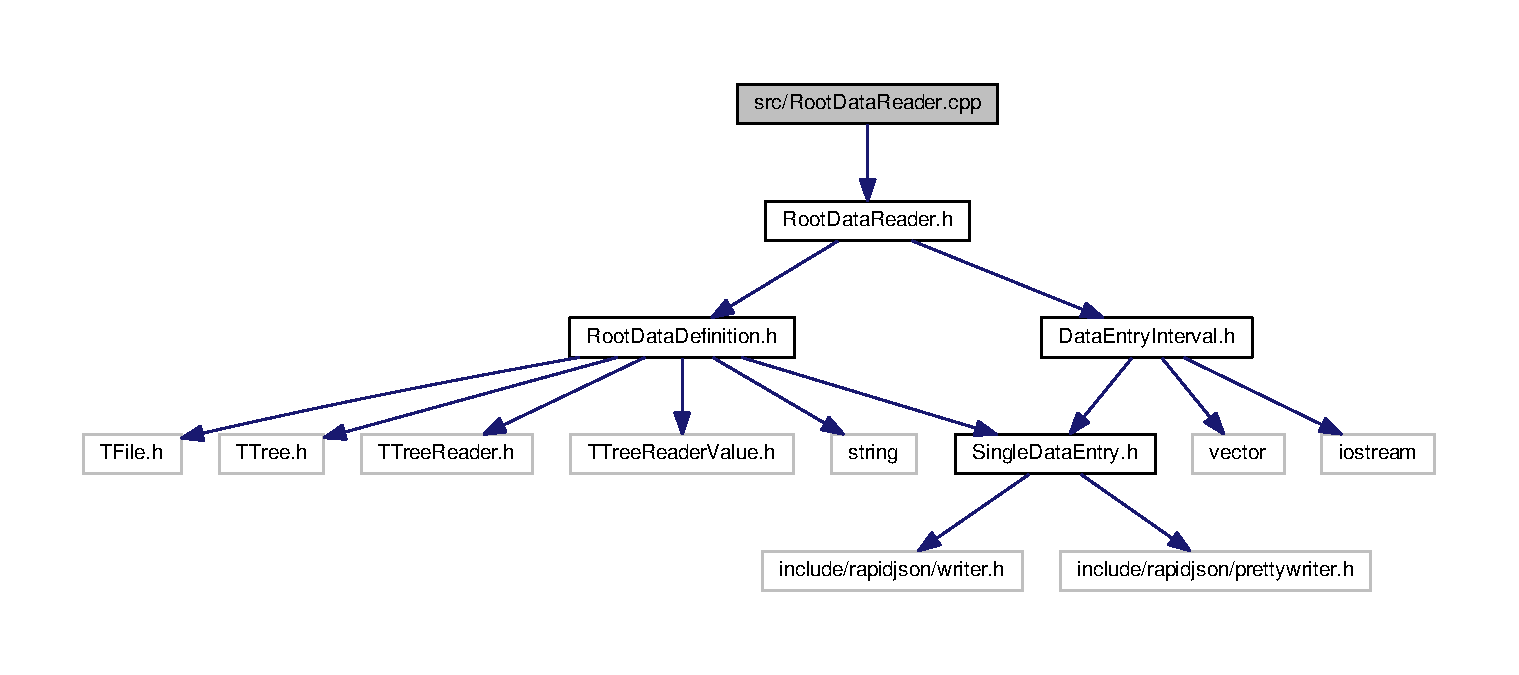
\includegraphics[width=350pt]{RootDataReader_8cpp__incl}
\end{center}
\end{figure}

\hypertarget{RootDataReader_8h}{\section{src/\+Root\+Data\+Reader.h File Reference}
\label{RootDataReader_8h}\index{src/\+Root\+Data\+Reader.\+h@{src/\+Root\+Data\+Reader.\+h}}
}
{\ttfamily \#include \char`\"{}Root\+Data\+Definition.\+h\char`\"{}}\\*
{\ttfamily \#include \char`\"{}Data\+Entry\+Interval.\+h\char`\"{}}\\*
Include dependency graph for Root\+Data\+Reader.\+h\+:\nopagebreak
\begin{figure}[H]
\begin{center}
\leavevmode
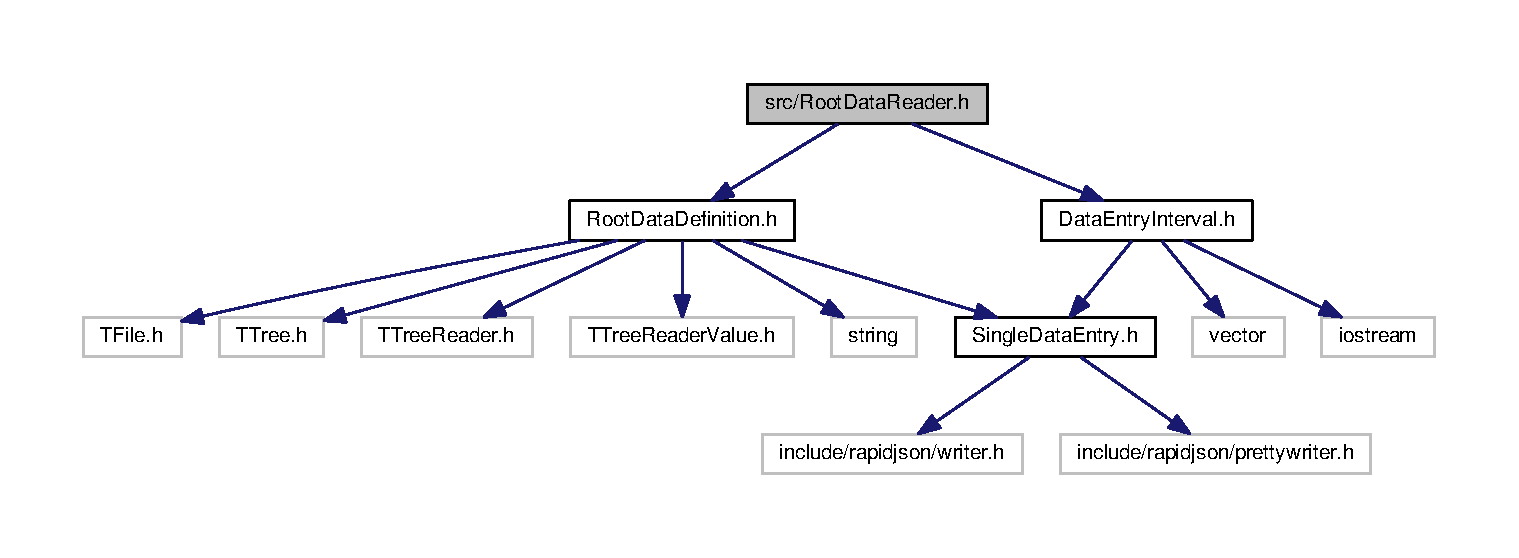
\includegraphics[width=350pt]{RootDataReader_8h__incl}
\end{center}
\end{figure}
This graph shows which files directly or indirectly include this file\+:\nopagebreak
\begin{figure}[H]
\begin{center}
\leavevmode
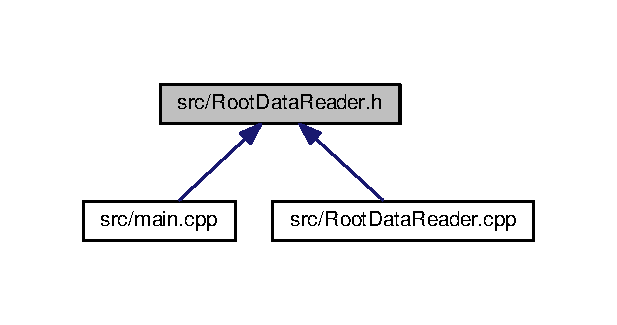
\includegraphics[width=296pt]{RootDataReader_8h__dep__incl}
\end{center}
\end{figure}
\subsection*{Classes}
\begin{DoxyCompactItemize}
\item 
class \hyperlink{classRootDataReader}{Root\+Data\+Reader}
\begin{DoxyCompactList}\small\item\em Class responsible for reading data of various structure in the R\+O\+O\+T format (T\+Tree within T\+File). \end{DoxyCompactList}\end{DoxyCompactItemize}

\hypertarget{SingleDataEntry_8h}{\section{src/\+Single\+Data\+Entry.h File Reference}
\label{SingleDataEntry_8h}\index{src/\+Single\+Data\+Entry.\+h@{src/\+Single\+Data\+Entry.\+h}}
}
{\ttfamily \#include \char`\"{}include/rapidjson/writer.\+h\char`\"{}}\\*
{\ttfamily \#include \char`\"{}include/rapidjson/prettywriter.\+h\char`\"{}}\\*
Include dependency graph for Single\+Data\+Entry.\+h\+:\nopagebreak
\begin{figure}[H]
\begin{center}
\leavevmode
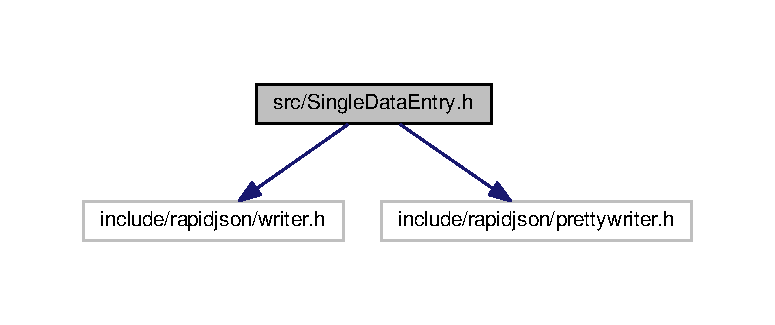
\includegraphics[width=350pt]{SingleDataEntry_8h__incl}
\end{center}
\end{figure}
This graph shows which files directly or indirectly include this file\+:
\nopagebreak
\begin{figure}[H]
\begin{center}
\leavevmode
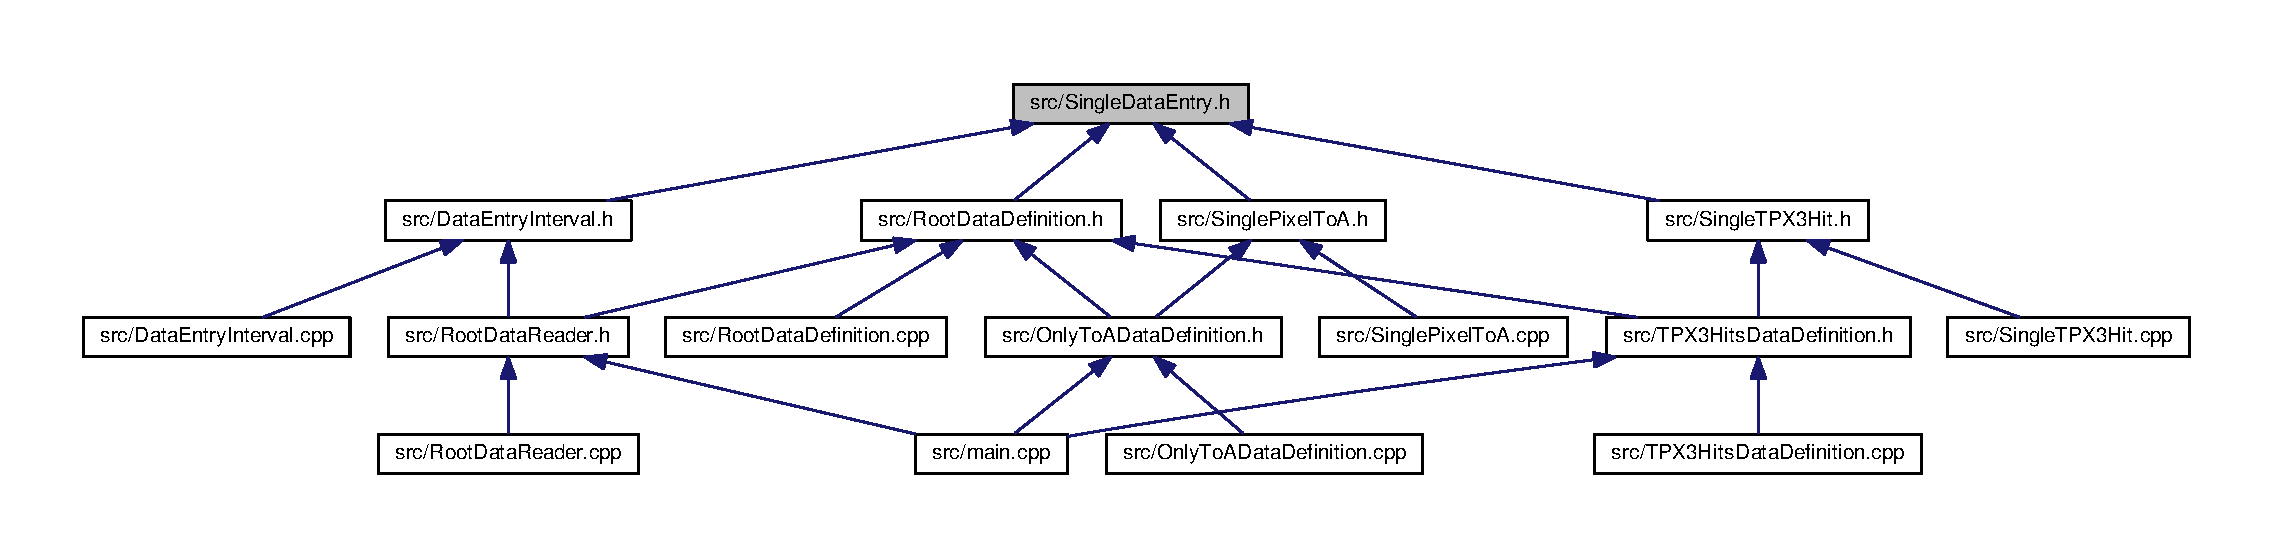
\includegraphics[width=350pt]{SingleDataEntry_8h__dep__incl}
\end{center}
\end{figure}
\subsection*{Classes}
\begin{DoxyCompactItemize}
\item 
class \hyperlink{classSingleDataEntry}{Single\+Data\+Entry}
\begin{DoxyCompactList}\small\item\em Abstract class representing a data object to be retrieved from the R\+O\+O\+T file. \end{DoxyCompactList}\end{DoxyCompactItemize}

\hypertarget{SinglePixelToA_8cpp}{\section{src/\+Single\+Pixel\+To\+A.cpp File Reference}
\label{SinglePixelToA_8cpp}\index{src/\+Single\+Pixel\+To\+A.\+cpp@{src/\+Single\+Pixel\+To\+A.\+cpp}}
}
{\ttfamily \#include \char`\"{}Single\+Pixel\+To\+A.\+h\char`\"{}}\\*
Include dependency graph for Single\+Pixel\+To\+A.\+cpp\+:\nopagebreak
\begin{figure}[H]
\begin{center}
\leavevmode
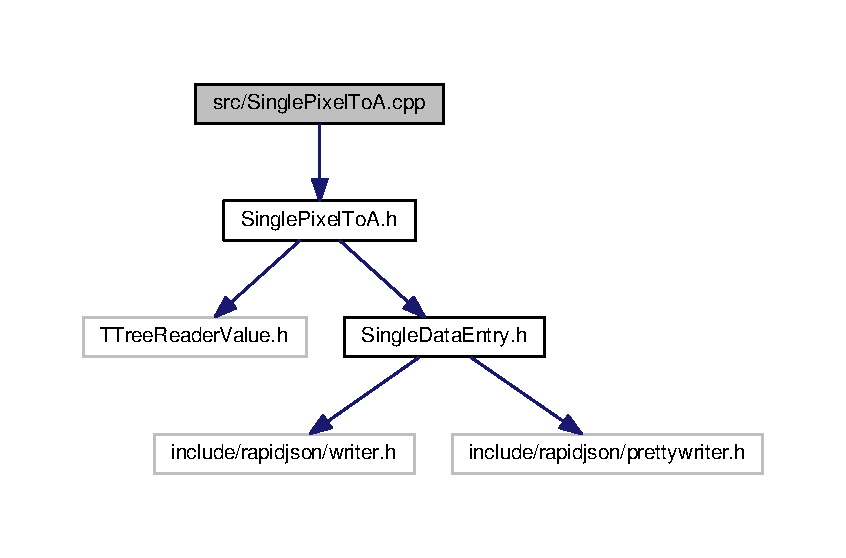
\includegraphics[width=350pt]{SinglePixelToA_8cpp__incl}
\end{center}
\end{figure}

\hypertarget{SinglePixelToA_8h}{\section{src/\+Single\+Pixel\+To\+A.h File Reference}
\label{SinglePixelToA_8h}\index{src/\+Single\+Pixel\+To\+A.\+h@{src/\+Single\+Pixel\+To\+A.\+h}}
}
{\ttfamily \#include \char`\"{}T\+Tree\+Reader\+Value.\+h\char`\"{}}\\*
{\ttfamily \#include \char`\"{}Single\+Data\+Entry.\+h\char`\"{}}\\*
Include dependency graph for Single\+Pixel\+To\+A.\+h\+:\nopagebreak
\begin{figure}[H]
\begin{center}
\leavevmode
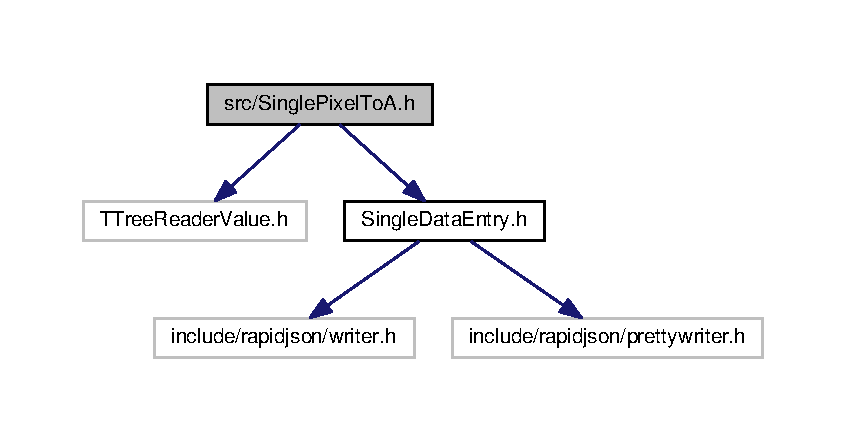
\includegraphics[width=350pt]{SinglePixelToA_8h__incl}
\end{center}
\end{figure}
This graph shows which files directly or indirectly include this file\+:\nopagebreak
\begin{figure}[H]
\begin{center}
\leavevmode
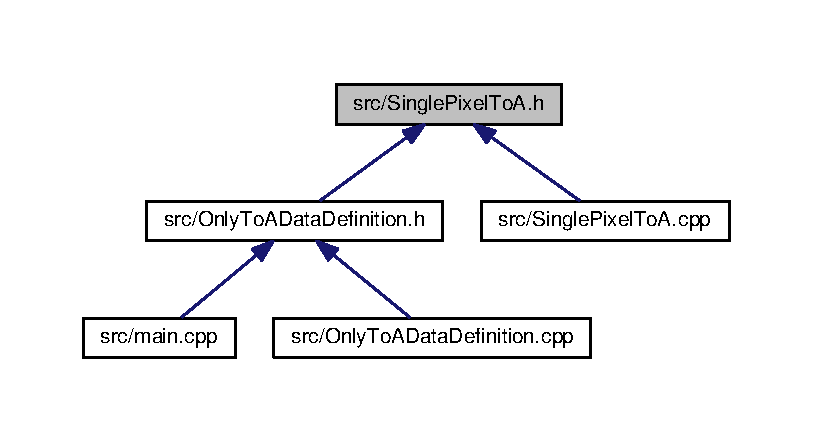
\includegraphics[width=350pt]{SinglePixelToA_8h__dep__incl}
\end{center}
\end{figure}
\subsection*{Classes}
\begin{DoxyCompactItemize}
\item 
class \hyperlink{classSinglePixelToA}{Single\+Pixel\+To\+A}
\begin{DoxyCompactList}\small\item\em Class defining the data object containing only single value (of type double) -\/ To\+A. \end{DoxyCompactList}\end{DoxyCompactItemize}

%--- End generated contents ---

% Index
\newpage
\phantomsection
\addcontentsline{toc}{chapter}{Index}
\printindex

\end{document}
